\documentclass[a4paper,twoside]{article}
\usepackage[a4paper]{geometry}
% \usepackage[a4paper,showframe]{geometry} % add showframe for debug
% \usepackage{titleps}
\usepackage[pagestyles]{titlesec}
\usepackage[all]{nowidow} % avoid orphan lines

% Extra colours; need to be first
\usepackage[usenames,dvipsnames,svgnames,table]{xcolor}

% Basic packages
\usepackage[utf8]{inputenc}
\usepackage[T1]{fontenc}

% Landscape mode
\usepackage{pdflscape}

% Additional font
\usepackage{FiraMono}

% Bibtex+cite
\usepackage{cite}
\usepackage{url}
\usepackage[nottoc,numbib]{tocbibind}

% URL
\usepackage[
  colorlinks=true,
  urlcolor=blue,
  citecolor=black,
  linkcolor=.
]{hyperref}

% Lists
\usepackage{scrextend}
\addtokomafont{labelinglabel}{\sffamily}
\usepackage[inline]{enumitem} % for enumerate* environment.

% Maths & symbols
\usepackage{mathtools}
\usepackage{amssymb}
\usepackage{pifont}

% Mono font
\usepackage[scaled]{beramono}

% Spacing
\usepackage{xspace}

% Graphics
\usepackage{graphicx}

% Markdown
\usepackage[
  definitionLists=true,
  tightLists=false,
  % blankBeforeCodeFence=true,
  fencedCode=true,
  footnotes=true,
  inlineFootnotes=true,
  hybrid=true
]{markdown}


% Table
\usepackage{booktabs}
\usepackage{tabularx}
\usepackage{multirow}

% Floating placement
\usepackage{placeins}
% use \FloatBarrier before a \section to ensure all floating are displayed
% before the new section

% Caption styling
\usepackage[justification=centering]{caption}

% Additional colours
\definecolor{c1}{HTML}{006C71}
\definecolor{c2}{HTML}{005155}
\definecolor{c3}{HTML}{FF8928}
\definecolor{c4}{HTML}{E86900}
\colorlet{ImportantCode}{ForestGreen}
\colorlet{ImportantCode2}{RubineRed}
\colorlet{ImportantCode3}{RedOrange}

% TIKZ & related packages/settings
\usepackage{tikz}
\usepackage{pgfplots}
\usetikzlibrary{shapes,fit,backgrounds,arrows,positioning,chains,patterns}
\pgfplotsset{compat = 1.14}

% for caching tikz pictures
% \usetikzlibrary{external}
% \tikzexternalize[prefix=tikz-figures/]
% \pgfrealjobname{tikz}


% Listings
\usepackage{listings,multicol}
\usepackage{lstscala}
\lstloadlanguages{[ANSI]C}

\lstdefinelanguage{C99}[ANSI]{C}{
  basicstyle=\ttfamily,
  commentstyle=\color{lstscalacmt},
  morekeywords={bool,int8\_t,int32\_t,uint32\_t},
  keywordstyle=\color{blue!30!darkgray}\bfseries,
  moredelim=**[is][\color{ImportantCode}]{@}{@},
  moredelim=**[is][\color{ImportantCode2}]{§}{§},
  moredelim=**[is][\color{ImportantCode3}]{£}{£},
}

\lstdefinelanguage{Leon}{ % Using `Scala` result in a infinite recursion
  style=scala-color,
  morekeywords={[2]Unit,Boolean,Byte,Int,BigInt,String,Char,true,false},
  %keywordstyle={[2]\color{blue!30!darkgray}\bfseries}
}

\newcommand{\Inline}[1]{\lstinline[basicstyle=\ttfamily]|#1|}
\newcommand{\InlineC}[1]{\lstinline[language=C99]|#1|}
\newcommand{\InlineS}[1]{\lstinline[language=Leon]|#1|}
% %\newcommand{\inlineScala}[1]{\lstinline[language=MyScala,breaklines=true,breakatwhitespace=true]|#1|}

% Use code in description item, Based on http://tex.stackexchange.com/a/181325/77356
\newcommand*{\lstitem}[1]{
  \setbox0\hbox{\textbf{\Inline{#1}}}
  \item[\usebox0]
}

% %\lstset{aboveskip=5pt,belowskip=10pt}
% \lstset{captionpos=b,abovecaptionskip=1em}

% For long listings
\lstdefinestyle{LongCode}{
  %aboveskip=1ex,
  % basicstyle=\small\ttfamily,
  basicstyle=\scriptsize\ttfamily,
  % basicstyle=\tiny\ttfamily,
  %belowskip=1ex,
  breaklines=true,
  postbreak=\raisebox{0ex}[0ex][0ex]{\ensuremath{\color{red}\hookrightarrow}},
  breakautoindent=false,
  %breakatwhitespace=false,
  %columns=fullflexible,
  multicols=2,
  framerule=0pt,
  framexrightmargin=0em,
  framexleftmargin=0em,
  % numbers=left,
  % numberstyle=\footnotesize\sffamily,
  tabsize=2
}


% Env for short code: no label, no caption and "inlined" with a box
\lstnewenvironment{ShortCode}[1]
    {
      \lstset{
        language=#1,
        frame=trBL % box the frame & double line on bottom and left side
      }
    }
    {
    }

% Env for longer code: label, caption and "floating" with a box
\lstnewenvironment{Code}[3]
    {
      \lstset{
        language=#1,
        label={#2},
        caption=#3,
        captionpos=b, % bottom
        float=!h,     % "here"
        frame=trBL,   % box the frame & double line on bottom and left side
        % frameround=tttt
      }
    }
    {
      % DEBUG:
      % 1: #1 \\
      % 2: #2 \\
      % 3: #3
    }



% Tables
% \newcommand{\heading}[1]{\multicolumn{1}{c}{\textbf{#1}}}
% \newcommand{\vheading}[1]{\rotatebox[origin=c]{90}{~\textbf{#1}~}}


% To centre table too wide
% credit: http://tex.stackexchange.com/a/27099/77356
\makeatletter
\newcommand*{\centerfloat}{%
  \parindent \z@
  \leftskip \z@ \@plus 1fil \@minus \textwidth
  \rightskip\leftskip
  \parfillskip \z@skip}
\makeatother



% General styling
\let\oldsection\section
\renewcommand\section{\cleardoublepage\oldsection}

% For some reason page margin are swapped when having a title page with a
% different geometry. We fix that manually by 1) swapping the margin and
% 2) swapping the page number position (page style)
% credit: http://tex.stackexchange.com/a/36016/77356
\makeatletter
\newcommand*{\flipmargins}{%
  \clearpage
  \setlength{\@tempdima}{\oddsidemargin}%
  \setlength{\oddsidemargin}{\evensidemargin}%
  \setlength{\evensidemargin}{\@tempdima}%
  \if@reversemargin
    \normalmarginpar
  \else
    \reversemarginpar
  \fi
}
\makeatother

\newpagestyle{mystyle_no_header}{
  \setfoot[\thepage][][]{}{}{\thepage}
}

\newpagestyle{mystyle}{
  % \sethead[][][\firsttitlemarks\ifthesubsection{\thesubsection~\subsectiontitle}{\thesection~\sectiontitle}]{\firsttitlemarks\ifthesubsection{\thesubsection~\subsectiontitle}{\thesection~\sectiontitle}}{}{}
  \sethead[\thesection~\sectiontitle][][]{}{}{\thesection~\sectiontitle}
  % \setfoot[][][\thepage]{\thepage}{}{}
  \setfoot[\thepage][][]{}{}{\thepage}
}

% Additional macros
\newcommand{\TODO}[1]{\textcolor{YellowOrange}{(#1)}} % for inline TODO
% \newcommand{\TODO}[1]{\underline{(#1)}} % for inline TODO, PRINTING
\newcommand{\GenC}{\emph{GenC}\xspace}
\newcommand{\URL}[2]{#2:\xspace\href{#1}{#1}}
\newcommand{\RefSec}[1]{Section~\ref{#1}}
\newcommand{\RefTable}[1]{Table~\ref{#1}}
\newcommand{\RefApp}[1]{Appendix~\ref{#1}}
\newcommand{\RefFig}[1]{Figure~\ref{#1}}
\newcommand{\RefCode}[1]{Listing~\ref{#1}}
\newcommand{\BigO}[1]{\mathcal{O}(#1)}




%%%

\title{Extending Safe C Support In Leon}

\date{January 2017}

\author{Marco Antognini}

\begin{document}

\newgeometry{centering}
\pagenumbering{gobble}
\maketitle

\vfill

\begin{abstract}

As hardware designs get more robust and efficient, software can solve a wider
range of challenges, each one more advanced than the previous one. The direct
consequence is that software complexity grows continuously. Despite being used
more frequently in development processes, traditional testing frameworks are not
enough to avoid flaws in programs. Moreover, many company concerned by the
security of their applications, especially in mission critical industries, spend
a considerable effort and amount of money to write robust software certified by
solid guidelines and standards. For embedded systems, MISRA C is a certification
process commonly used that provides directive to write portable and maintainable
C code while avoiding many pitfalls of the language.

Leon takes an orthogonal approach by providing tools for formal verification of
programs written in a subset of Scala. In a previous work we introduced \GenC, a
module for Leon that converts Scala applications into equivalent and safe C99
programs, allowing developers to leverage high-level feature of Scala to
implement robust applications even for embedded systems.

The aim of this project is to augment Leon and \GenC in order to support a
larger fragment of Scala that includes inheritance, generic programming,
additional numeric types, pattern matching and more. Additionally, we closely
analyse the MISRA Guidelines and shape the generated C code to work towards
compliance with its rules while taking advantage of the verification
capabilities of Leon to automatically detect a variety of bugs. We discuss these
improvements and new features by implementing the famous LZW
compression/decompression algorithm as well as a kernel-based image processing
algorithm and show that the produced native C programs are significantly more
efficient both in terms of memory usage but also in terms of execution speed.

\end{abstract}

\vfill

\begin{center}
    Master Thesis Project under the supervision of \\
    Prof. Viktor Kuncak \& Régis Blanc \\
    Lab for Automated Reasoning and Analysis LARA - EPFL
\end{center}

\begin{center}
    
\includegraphics[width = 40mm]{res/epfl-logo}
\end{center}

\clearpage\null\newpage


\restoregeometry              %% restore the layout
\flipmargins
\pagestyle{mystyle_no_header}
\pagenumbering{arabic}

\tableofcontents
% \lstlistoflistings


\clearpage
\pagestyle{mystyle}

\section{Introduction}

Software become significantly more complex, solving every day new challenges,
partly thanks to the decrease in price of hardware which is constantly improved,
making computers more and more robust, quicker and more energy efficient.
Constant breakthroughs enabled us to revolutionise how people benefit from their
personal computers, or electronic devices in a general sense: from the
information now instantaneously available at our finger tips provided by
satellites orbiting our planet in an environment ranging from extremely cold to
scorching temperature with intense radiations, through remote devices performing
advanced scientific experiments at an incredibly huge distance from us
communicating using channels resilient to immense delay and numerous data
errors, to surgical and medical tools helping to understand and to fight
devastating diseases, for example using brain or heart implements to improve
patients' life.

Future technologies can be expected to follow a similar evolution, making
obvious that systems complexity is predicted to increase. Many companies already
spend a considerable amount of money to assert their software is exempt of life
threatening bugs through various certifications or to keep their data safe and
available in a matter of milliseconds. Hence, being able to evaluate the quality
of software, detecting issues before they arise, in a reliable and simple
fashion can significantly boost performance of Quality Assurance (QA) processes.

Development strategies were developed to actively reinforce software. They can
involve continuous integration servers to constantly check for defects by means
of regression or unit tests and powerful static analysers. Or they can be based
on general design techniques, such as employing design-by-contract programming
or runtime validations and exception mechanisms.

\begin{figure}[!h]
  \centering
  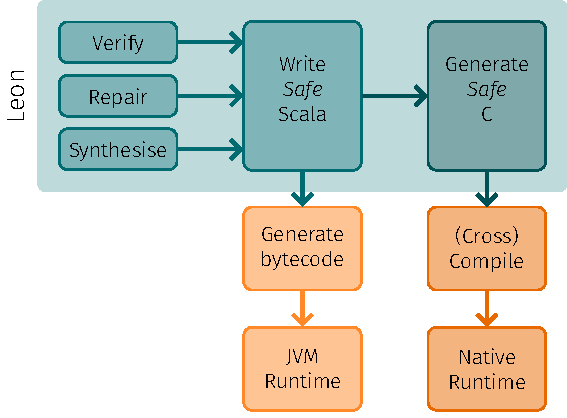
\includegraphics{res/dev_process.pdf}
  \caption{Development Process}
  \label{fig:dev-pipeline}
\end{figure}

For programs written in Scala, Leon \cite{leonweb} is a powerful instrument that
works at solving this general issue of quality by providing tools to verify
contracts, repair erroneous implementations or even synthesises code. However,
because Scala is based on JVM runtime, such tools are close to worthless for
many companies that run their software on very small devices: the lack of memory
and CPU resources prevents running virtualised code on such hardware. This
explains why those systems are written in low-level, native languages often
taking their roots in the C language.

For these reasons we have previously introduced the \GenC module of Leon
\cite{genc1} to transpile Scala programs into a safe and equivalent C99 pieces
of software. \GenC allows programmers to leverage the high-level features of the
Scala programming language and reduce the development cost of low-level software
while avoiding using error-prone languages. Moreover it helps developers avoid
some of the most commonly reported bugs (e.g. buffer overflows or arithmetic
errors).

The overall, high level development pipeline is illustrated in
\RefFig{fig:dev-pipeline}. The first step is to generate a valid and verified
Scala program using Leon. Then the program can be converted into an equivalent
C99 code through the \GenC phase.  The produced code can then be compiled using
any standard-compliant C99 compiler -- for example Clang \cite{clang}, GCC
\cite{gcc} or formally verified compilers like CompCert \cite{Leroy-backend}
\cite{compcert} -- to generate a native and optimised assembly code for specific
hardware architectures. Then the compiled program can be shipped to the desired
hardware and executed as usual.

I first introduced \GenC through an \emph{Optional Semester Project} at EPFL.
The work presented in this report is a continuation of this initial project in
the form of my \emph{Master Thesis Project}. Both projects were supervised by
the \emph{Lab for Automated Reasoning and Analysis} (LARA).

The present work adds to \GenC a better support for object oriented or generic
programming, a wider range of supported primitive types, an improved handling of
arithmetic expressions and an interfacing system to integrate existing
libraries, just to name a few. Together these improvements augment the range of
the supported fragments of Scala. We also introduce a new memory model based on
our analyse of recent improvements made to the \emph{xlang} module
\cite{Blanc:2013:OLV:2489837.2489838} \cite{xlang} regarding mutability. One
singular feature of this model is that it is solely based on stack allocation.

Furthermore, we studied reliability processes used for development of
applications targeted at embedded devices, such as the ones used in the
automotive industry. This work resulted in a re-engineering of \GenC to work
toward compliance with the MISRA Guidelines, which is intended to bring in
robustness and reliability to the software, and to empower users with more
static analysis tools. We discuss in this document how verification can help
substantially reduce the amount of bugs in programs and report on how the Leon
ecosystem manages to produce safe code free of undefined behaviour and under
which assumptions.

We also present two implementation of the famous LZW \cite{welch1985high}
compression and decompression algorithm, as well as some image manipulations
based on filters, illustrating how \GenC can successfully be used for real-life
applications to produce highly efficient native programs that are significantly
faster than the default JVM-based runtime offered by Scala.

We structure this report as follow. First we finish this section by reviewing
some related works. In \RefSec{motivation} we highlight the most common kinds of
bugs and what are the main challenges for embedded development. Then, we present
new features we developed for Leon itself in \RefSec{leon_features}. We
introduce the memory model on which the generated C99 code is relying on in
\RefSec{memory_model} and further discuss specific details of the translation
from Scala down to C in Sections \ref{translation_defs} and
\ref{translation_exprs}. Next, we specify how external libraries can be
integrated into the translation process in \RefSec{library}. In \RefSec{MISRA}
we present the MISRA Guidelines, discuss its importance and explain how Leon and
\GenC work toward compliance. Then, we showcase in Sections \ref{lzw} and
\ref{img_proc} the abilities of \GenC by implementing the LZW algorithm and some
image processing algorithm. We summarise this report in \RefSec{conclusion} and
in the final \RefSec{future_works} we introduce how Leon and \GenC can be
further improved to help developing safe applications.

\subsection*{Related Works}

Because \GenC spans several fields it is relevant to identify whether some
existing project proposes to transpile a high-level language into
embedded-friendly equivalent code, what kind of verification systems exist or
how bugs are tracked down in compilers.

First, we note that \GenC is not the first attempt to translate a high-level
language down to C. There exists, for example, the now discontinued java2c
\cite{java2c} project which claims to transpile a limited fragment of Java to C.
The free GNU Compiler for Java (GCJ), which is now discontinued as well and has
been removed from the GNU Compiler Collection (GCC), was designed to be capable
of emitting both bytecode and machine code. However, contrary to those two
projects, \GenC is built into a wider ecosystem that makes such translation even
more meaningful thanks to the different modules of Leon.

FLEX \cite{flex} was a compiler infrastructure for Java that featured program
analysis and optimisations for distributed and embedded systems with native
backends for StrongARM and MIPS processors. It was also capable of producing C
code, but unlike \GenC all its backends relied on a garbage collector at
runtime.

\GenC works on Scala programs, which would, if run as-is, require a full-fledged
Java Virtual Machine to be executed. There exists however some version of Java
and its virtual machine that are significantly lighter such as the JavaCard
system \cite{javacard}, which can run on microprocessor. Compared to C, this
subset of Java offers a better portability system with its well-defined runtime
and standard library. However, these advantages are limited by issues of
performance and memory size.

Recently started, the Scala Native project \cite{scala_native} already offers
the ability to compile many Scala programs into native assembly instructions
using the LLVM compiler and its internal representation language. \GenC differs
from Scala Native in several ways. First, unlike the assembly produced by Scala
Native, the generated C99 code can be inspected easily and therefore approved by
security teams when necessary. Second, by generated standard C code, we give the
user the opportunity to choose their C compilers, as well as the targeted
architecture for runtime and other environment tuning options that are not
exposed by Scala Native. Then, \GenC also takes into consideration verifications
of programs, and the limitations that the verification process imposes on the
Scala language, to produce efficient code that doesn't require garbage
collecting and other heavy runtime facilities that Scala Native deals with.

Frama-C \cite{framac} is somewhat similar to the static analysis modules of
Leon. Both offer to verify without actually running programs whether some
properties hold or not. But while Leon works with programs written in Scala,
Frama-C analyses software in C, which means that higher level concepts such as
inheritance or generic types cannot be used to design complex programs,
therefore limiting developers to basic tools. That being said, adding assertions
and properties written in ANSI/ISO C Specification Language (ACSL) \cite{acsl},
which interface nicely with C since it can be embedded in standard comment
block, to the generated C99 code based on the original verification conditions
the user wrote in Scala would be beneficial to help prove the new, low-level
program still respects its original specification.

Microsoft has also been working on a similar project to Frama-C called VCC
\cite{vcc}, with a major difference being that VCC works at verifying concurrent
C programs. The sub-language used to specify verification conditions is
significantly different, yet has no impact on runtime as well. It is not clear
whether this project is still active or not, but contrary to VCC \GenC does not
offer the ability to work with concurrent programs written in Scala.

The Cyclone programming language \cite{cyclone} was designed based on C to bring
safety to the language using a similar syntax, avoiding bugs such as buffer
overflows, format string attacks, dangling pointer accesses, and so forth. It
added support for exceptions, region-based memory management as well as an
optional garbage collector on top of the usual manual memory management of C.
Cyclone is now discontinued but several of its concept made their way into the
Rust system programming language. To the contrary, \GenC produces pure C99
programs, which are exempt of dangling pointers, while still being able to
detect any potential buffer overflow, thanks to Leon.

Finally, to design any program bigger than a few assembly instructions one will
need to use a compiler for whatever language is being used. \GenC indirectly
relies on project such as Csmith \cite{csmith} to improve the quality of
compilers, especially the C ones, in order to test its ability to produce valid
C. While \GenC currently only relies on classic regression tests, it could be
interesting to use a similar generator of random test-case than the one used by
Csmith to further assess its ability to transpile Scala code.


\section{Motivation}
\label{motivation}

% - give examples of bugs that have negative/positive impact
% - illustrate the difficulty of writing correct C code
% - introduce MISRA and why it is used in practice
% - give overview of how \GenC works

We begin this report by exposing how frequent and dangerous bugs can be through
diverse examples and issue databases. The second part of this section further
details which additional challenges need to be addressed when working with
embedded devises, introduce the MISRA Guidelines used by the industry to
certify the quality of programs and how \GenC fit in this certification process.


\subsection{A History of Bugs}
\label{bug_history}

There are some well-known bugs in the history of computer science that caused
major monetary loss to companies, and in a few cases even caused physical
injuries or death. But there also exist countless bugs that are more moderate
but still threaten the security of our information systems and everyday
computers. In some specific cases bugs evolved into features, and in
particularly odd cases vulnerabilities were abused to patch the software itself.
Here are a few examples:

\begin{description}

\item[Killer Bug, Therac-25]

The Therac-25, which was used in the 80's for radiation therapy, caused 6 known
accidents involving massive overdoses resulting in severe injuries and deaths. An
integer used to track error count overflowed, causing the program to re-enter a
valid state for operation~\cite{Leveson:1993:ITA:161477.161479}.

To fight against such bugs we instrumented Leon to check for potential integer
overflow without running the software.

\item[(s)elf-exploitation]

From time to time, a bug happen to be situated in the right position to
workaround another limitation. J. Garret explained in~\cite{self_exploitation}
how a buffer overflow was used to patch a game in the most unexpected way. He
also acknowledges that this wouldn't have been needed were the software
including a remote patch procedure.

\item[Out-of-Bounds Access \& Buffer Overflow]

Some of the most frequent kinds of bugs present in our software are overflows;
for example Apple Security Update HT207275~\cite{HT207275} patches several bugs
of which roughly 20\% were \emph{simple} buffer overflows and out-of-bounds
accesses.

Those are typically bugs that can be avoided using Leon and \GenC: the
verification procedure highlight place in Scala programs where overflows
can occur, with an example of values that triggers the bug at runtime.

\end{description}

According to the widely adopted \emph{Common Vulnerabilities and Exposures}
(CVE) database~\cite{cve}, which describes itself as \textit{The Standard for
Information Security Vulnerability Names} and has over 80,000 registered
tickets, buffer overflows account for approximately 10\% of the reported bugs
and integer overflows for roughly 1.6\%.

The \emph{CVE Details} website~\cite{cvedetails} reports that overflows, in its
general meaning, is third in a vulnerabilities-by-type ranking. One might expect
that overflows are sufficiently studies and known by developers that their
presence in our modern software should not contain many such bugs. However, as
depicted by \RefFig{fig:bug_stats}, the fact is that the general trend is not
toward a reduction of the number of discovered bugs in this category. After a
closer reading of the CVE entries it appears that many vulnerabilities
categorised as \emph{Denial of Service} or \emph{Execute Code} are also tagged
as \emph{Overflow}.

It follows that people need clever tools, such as Leon, to detect and eradicate
those omnipresent issues.

\begin{figure}
\centering

\begin{tikzpicture}
\begin{axis}[
    % title={The 3 most frequent categories of bugs in the last 10 years},
    xlabel={Years},
    ylabel={Number of Vulnerabilities},
    ymin=0, ymax=3000,
    xtick={2006,2007,2008,2009,2010,2011,2012,2013,2014,2015,2016},
    xticklabel style={rotate=80},
    x tick label style={/pgf/number format/.cd,%
      scaled x ticks = false,
      set thousands separator={},
      fixed
    },
    xlabel shift=1pt,
    legend pos=north east,
    legend cell align=left,
    legend entries={Execute Code,Denial of Service,Overflow},
    ymajorgrids=true,
    grid style=dashed,
    width=0.95\textwidth,
    height=8cm,
]

\addplot[
    color=red,
    % mark=square,
    ]
    coordinates {
    (2006,2719)(2007,2601)(2008,2310)(2009,2185)(2010,1714)(2011,1334)(2012,1457)(2013,1186)(2014,1573)(2015,1820)(2016,1494)
    };

\addplot[
    color=black,
    % mark=circle,
    ]
    coordinates {
    (2006,893)(2007,1100)(2008,894)(2009,1035)(2010,1102)(2011,1221)(2012,1425)(2013,1454)(2014,1559)(2015,1792)(2016,2029)
    };

\addplot[
    color=blue,
    % mark=triangle,
    ]
    coordinates {
    (2006,662)(2007,953)(2008,699)(2009,700)(2010,678)(2011,770)(2012,842)(2013,859)(2014,850)(2015,1079)(2016,1326)
    };

\end{axis}
\end{tikzpicture}

\caption{The 3 most frequent categories of bugs in the last 10 years. Source:
\cite{cvedetails}}
\label{fig:bug_stats}

\end{figure}

\subsection{Challenges for Embedded Devices}

Seen the range of bugs and their frequencies and gravity, it appears clear that
developers needs good tools in order to write decently safe software. Embedded
devices add to this context the challenge of producing safe \textbf{and}
efficient code with a limited amount of resources, such as computational speed,
memory capacity and energy consumption. C is commonly chosen to develop programs
for such restrictive environments. The reason for this choice is twofold.
Firstly, in contrast to Java or Python it is a native language and therefore is
more suited for such tiny runtime environments. Secondly, despite the work of
many C++ developers C remains the preferred language in practice with an
adoption of 60\%~\cite{saks}, certainly for historical reasons but also because
most suspect that \textit{high-level} language features such as meta-programming
or object oriented design are too greedy.

However, it is well-known that C is not an easy language and that many pitfalls
make developers' life hard. Furthermore, if one wants to write portable
software, one has to work through numerous language elements that are either
implementation-defined or described as undefined behaviour by the C Standard. To
get an idea of the difficulty this represents, the C99 Standard \cite{c99} in
its Annex J holds a bullet-point list of such undefined elements that is 13
pages long.

The following example is one of the shortest function that can trigger undefined
behaviour, illustrating the extend to which the language is
implementation-defined:

\begin{ShortCode}{C99}
int foobar(int x) { return -x; } // undefined when x == INT_MIN
\end{ShortCode}

It is not obvious in this snippet what is the ranged covered by \InlineC{int}:
the C99 standard specifies a minimal size for \InlineC{int} but leaves the
implementation define its size as well as its memory representation, with some
constraints. It could theoretically be defined as a 19-bit integer using 1's
complement representation.

On the other end of the spectrum, the Java programming language and its virtual
machine, and therefore Scala, precisely define the range of \InlineC{int} (or
\InlineS{Int} in Scala) and its memory representation as a 32-bit integer using
the now standard 2's complement representation. Moreover, the behaviour of the
unary minus operator is properly defined by the Java Standard \cite{java8} on
the whole $[-2^{31}, 2^{31}-1]$ range using wrap around semantic for overflow,
meaning that $-(-2^{31}) \equiv -2^{31}$.

On top of the C standard, many companies, especially in the car, aeronautic or
medical industries, adopt additional guidelines to improve the quality of their
software. They tend to be very strict and even forbid some of the language
features deemed unsafe or unpredictable. One of the most used set of rules is
\emph{MISRA C: Guidelines for the use of the C language in critical
systems}~\cite{misra}.

Among many things, the MISRA Guidelines forbid any kind of dynamic memory
allocation, leaving only static allocation available to the developers and
therefore significantly limiting program designs; the rationale being that heap
allocation is hard to predict not only in terms of available memory space but
also, and this is equally important for real-time application, in term of
responsiveness~\cite{gross} and is therefore inadequate for most embedded
systems.

One of the direct consequences of this memory allocation model is that a
traditional \InlineS{List} in Scala cannot be implemented trivially in C.
Listings \ref{lst:IntListScala} and \ref{lst:IntListC} illustrate this.

% // A list over integer as one would define for Leon
\begin{Code}{Leon}{lst:IntListScala}{List of integers in Scala.}
abstract class List
case class Cons(x: Int, tail: List) extends List
case class Nil() extends List
\end{Code}

% // A simple link list in C with heap allocation
\begin{Code}{C99}{lst:IntListC}{List of integers in C using heap allocation.}
#include <inttypes.h>
#include <stddef.h>
#include <stdlib.h>

typedef struct List List;
struct List { int32_t x; List* tail; };
static List* const NIL = NULL;

List* cons(int32_t x, List* tail) {
  // This might fail or take an arbitrary long time to execute.
  List* head = malloc(sizeof(List));
  head->x = x;
  head->tail = tail;
  return head;
}

void release(List* list) {
  if (list != NULL) {
    // This recursion could blow up the stack.
    release(list->tail);
    free(list);
  }
}
\end{Code}

With \GenC, developers can use Leon produce low level C99 code as safe as the
verified Scala program given as input without having to deal with portability
issues. By using a language like Scala, programmers can take advantage of the
strong type system to avoid illegal type conversions that emerge from the needs
of \InlineC{void*} in C due to the absence of generic types, but also benefit
from the well-defined nature of the language.

Additionally, we believe it is possible to write safe \textbf{and} efficient
code, as we hint with the example of \RefCode{lst:appends}. We can write two
different \InlineS{append} functions for a list of fixed maximum capacity. One
with a wide contract that returns an error when the list is already full and the
other one with a narrow contract that appends the element without checking the
capacity but should be called exclusively on non-full lists. With Leon, we can
ensure that calls to the optimised version are valid, without incurring runtime
cost for assertions, and therefore allow the developer to follow the C motto
``not paying for what you don't use'' without any additional risk.

\begin{Code}{Leon}{lst:appends}{Optimisation through verification}
case class ArrayList(val buffer: Array[Int], var size) {
  require(0 <= size && size <= buffer.length)

  def appendSafe(x: Int): Boolean = {
    if (size < buffer.length) {
      buffer(size) = x
      size += 1
      true
    } else false
  }

  def appendOptimized(x: Int): Unit = {
    require(size < buffer.length) // Only checked statically.
    buffer(size) = x
    size += 1
  }
}
\end{Code}


\section{Additional Features For Leon}
\label{leon_features}


We introduce in this section new tools for Leon that aim at increasing the
safety of Scala programs, allowing Leon to handle a larger fraction of the Scala
programming language and providing users with I/O operations through a safe API.

\subsection{Strict Arithmetic Model \& 8-bit Integer}

% - Introduction of Byte w/ integer type promotion for common operations
%    + explain type promotion rules;
%    + included in AST to make sure every module follows the Java convention
%      correctly.


The verification facilities of Leon were augmented in two ways. Firstly,
\InlineS{Byte} is now supported in addition to \InlineS{Int} and
\InlineS{BigInt}. Secondly, we have introduced the \Inline{--strict-arithmetic}
option to help detect unexpected or undesired behaviour in the source code in
order to avoid many runtime bugs.

\subsubsection*{8-bit Integer Support}

The smallest integer available in Java and Scala is \InlineS{Byte}. It is
specifically defined as a 8-bit signed integer using 2's complement
representation and therefore can represent any integer in the asymmetric range
$[-128,127]$. Furthermore, arithmetic operations on \InlineS{Byte} and
\InlineS{Int} (and any other primitive type) is fully defined by the Java
specification~\cite{java8}.

In order to introduce into Leon support for \InlineS{Byte} we decided to
explicitly include in the Abstract Syntax Tree (AST) representing programs the
different integer promotion rules defined by Java that are followed by Scala as
well. This has the advantage to encode those rules in one place only (i.e. when
extracting a program into its AST form) such that no other module of Leon needs
detailed knowledge of the nature of integer arithmetic.

For the current scope of Leon, the integer promotion rules consist of:

\begin{enumerate}

\item widening \InlineS{Byte} to \InlineS{Int} (i.e. adding 24 leading bits such
that the newly created integer represent the same value) when a \InlineS{Byte}
is involved in any arithmetic operation, and

\item narrowing \InlineS{Int} to \InlineS{Byte} (i.e. keeping only the 8
least-significant bits) when the integer is explicitly truncated.

\end{enumerate}

The Java integer promotion rules impose that a \InlineS{Byte} is automatically
widened to an \InlineS{Int} before carrying out any arithmetic operations, even
for the bitwise negation (\InlineS{\~}) operator which therefore produces 32-bit
integers as if one would have written \InlineS{\~(b.toInt)}. However, narrowing
casts are always explicitly introduced with the \InlineS{toByte} method of
\InlineS{Int}.

We detail in the \RefSec{primitive_type} how \InlineS{Byte} support is
implemented in \GenC.

\subsubsection*{Strict Arithmetic Checking}

% - Introduction of more overflow (initiated by Regis) \& strict arithmetic
%   checks for common operations.
%    + why <<, >>, >>> rhs is checked (non intuitive behaviour even if well
%      defined);
%    + more overflow checking to catch corner cases + not well defined code under
%      C standard (e.g. \%).

It is common knowledge that division by 0 in Java triggers a
\InlineS{java.lang.ArithmeticException} and Leon has been emitting verification
issues when such a dangerous instruction could be triggered in the user code.
Furthermore, Java specifies exactly how should \InlineS{Int.MinValue} be
transformed by the unary minus operator on the asymmetric range
$[-2^{31},2^{31}-1]$: the JVM should precisely yield \InlineS{Int.MinValue} and
not throw any exception. Because this behaviour is not obvious and could lead to
bugs in a software we have introduced a more strict verification mode, available
with the \Inline{--strict-arithmetic} option, that automatically instruments the
input source code to detect the following potentially undesired situation (where
\InlineS{x} and \InlineS{y} both denote \InlineS{Int} values):

\pagebreak[4]
\begin{enumerate}

\item Overflows (also independently available with the \Inline{--overflow} option)

  \begin{enumerate}

  \item \InlineS{-x}, when \InlineS{x} is \InlineS{Int.MinValue};

  \item \InlineS{x + y}, when the values of \InlineS{x} and \InlineS{y} produce
  an overflow;

  \item \InlineS{x - y}, when the values of \InlineS{x} and \InlineS{y} produce
  an overflow;

  \item \InlineS{x * y}, when the values of \InlineS{x} and \InlineS{y} produce
  an overflow;

  \item \InlineS{x / y}, when \InlineS{x} and \InlineS{y} are
  \InlineS{Int.MinValue} and \InlineS{-1}, respectively;

  \end{enumerate}

\item Undesired behaviour

  \begin{enumerate}

  \item \InlineS{x \% y}, when \InlineS{x} and \InlineS{y} are
  \InlineS{Int.MinValue} and \InlineS{-1}, respectively.

  While the result is very well defined in Java and Scala and one can
  understandably expect an answer of 0 this is not well defined in C99 and is
  actually undefined in C11~\cite{regehr}. This is why we treat is as undesired
  behaviour with the \Inline{--strict-arithmetic} option.

  \item \InlineS{x >> y}, \InlineS{x >>> y} or \InlineS{x << y} when \InlineS{y}
  is outside the range$[0,31]$.

  In Java and Scala only the 5 lowest-order bits of \InlineS{y} are considered,
  effectively mapping \InlineS{y} onto $[0,31]$ using modulo arithmetic. Not
  only is the behaviour undefined in C99 when \InlineS{y} is outside of this
  range but we believe this behaviour to be always undesired and therefore
  unsafe.

  \end{enumerate}
\end{enumerate}

Although \InlineS{x << y} can, and very often will, overflow we believe that
this behaviour is actually intended when manipulating bit patterns. For signed
integer in C99, such overflow are however undefined. We detail in
\RefSec{shifts} how we deal with this issue when generated equivalent and safe C
code.

The overflows detected here can partially be detected at runtime in a Java
program by using the \InlineS{negateExact}, \InlineS{addExact},
\InlineS{substractExact}, and \InlineS{multiplyExact} methods of
\InlineS{java.lang.Math} \cite{java8math}. It however appears that no such
built-in method exists for detecting overflows in divisions.

The extra assertions added by \Inline{--strict-arithmetic} are assumed to be
verified when converting the Scala code into C by \GenC in order to avoid
triggering undefined behaviour when running the generated C code.


\subsection{I/O Framework}
\label{io_framework}

While most embedded systems do not have file I/O it remains an important feature
for many programs. That is why we have introduced I/O support for both standard
input and output streams and files in Leon's library. We describe here the
relevant features of the \InlineS{leon.io} package for \GenC.

This framework serves also as a proof of concept for using C library functions
and types with \GenC. We further discuss this point in \RefSec{library}.

\begin{description}

\lstitem{leon.io.StdOut}

One case use the \InlineS{StdOut} object in order to read data from the standard
input stream. Specifically, it is possible to print, with or without a new line,
\InlineS{String}, \InlineS{Char}, \InlineS{Byte} and \InlineS{Int} with the
\InlineS{print} and \InlineS{println} functions.

\lstitem{leon.io.StdIn}

Similarly, the \InlineS{StdIn} object provides facilities to read data from the
standard input stream. For reasons exposed in \RefSec{primitive_type}, it is
currently only possible to read \InlineS{Int} and \InlineS{Byte}.

Two flavours are available: \InlineS{readInt} (\InlineS{readByte}) and
\InlineS{tryReadInt} (\InlineS{tryReadByte}). The first one always returns a
number and therefore should only be used when one can trust the input source to
be valid. The other one returns a \InlineS{leon.lang.Option} in order to
distinguish success reads from failures such as reaching the end of the input
or, in the case of \InlineS{tryReadInt}, attempting to read something that
doesn't match the format of an \InlineS{Int}.

In order to provide equivalence between C and Scala we implement those functions
such that they follow the C conventions on byte and 32-bit decimal integer
format, skipping any leading space for the latter as \InlineC{scanf("\%d", &x)}
would assuming 32-bit integers. That is, we accept integers that match the
following regular expression: \Inline{\\s*[+-]?\\d+}. For simplicity reasons, we
leave handling of overflows as undefined.

A curious reader might wonder why the provided functions take an implicit
\InlineS{State} parameter: \InlineS{def readByte()(implicit state: State): Byte
= ...}. This is an artefact for verification purposes \cite{xlang}: it ensures
that calling such methods can produce different results every time.

\lstitem{leon.io.FileOutputStream}

To print content to a new file, we provide \InlineS{FileOutputStream}. It
provides functions to check whether the file was successfully opened and the
ability to write \InlineS{String}, \InlineS{Char}, \InlineS{Byte} and
\InlineS{Int} at the end of the file through the \InlineS{write} overloaded
method which requires the stream to be open and report errors by returning
\InlineS{false}.

It is important to note that one should always invoke the \InlineS{close()}
method when the file stream is no longer needed in order to let the underlying
system reclaim file resources.

\lstitem{leon.io.FileInputStream}

Like \InlineS{StdIn}, \InlineS{FileInputStream} provides an API to read
\InlineS{Byte} and \InlineS{Int}, but from a file. The \InlineS{readByte},
\InlineS{readInt}, \InlineS{tryReadByte} and \InlineS{tryReadInt} methods
follows the same convention as detailed above, plus require that the file is
open. Finally, one should also call \InlineS{close()} when the file stream is no
longer used to avoid leaking resources.

\end{description}

\section{Memory, Aliasing \& Mutability Models For \GenC}
\label{memory_model}
\label{aliasing}
\label{mutability}

In the previous section we discussed how Leon was extended to support more Scala
programs with additional verification conditions to enforce a higher quality of
software. We now continue the discussion of overall feature support in
Leon/\GenC by exposing the memory model used by the generated C code, and which
limitations we impose in addition of the restrictions required by Leon.

Thanks to the \emph{xlang} module of Leon it is possible to transform a large
set of imperative programs into a functional equivalent and to verify such
programs. With \GenC we however want to keep the imperative nature of the input
code in order to produce as efficient as possible C code. To achieve this we do
not apply this transformation to the Abstract Syntax Tree (AST), yet we retain
the same restrictions on the supported imperative features because one of the
requirement of \GenC is that the input program must be valid and therefore
verified.

On the one hand, \emph{xlang} allows one to use local \InlineS{var}ibables,
assignments, blocks, \InlineS{while} loops (with \InlineS{invariant}),
imperative arrays (i.e. array elements can be mutated) and mutable objects (i.e.
classes with fields declared using \InlineS{var}).

On the other hand, it forbids most form of aliasing: in any given scope no two
named objects (i.e. local variable, function parameter or class member) can
refer to the same memory area. To ensure no aliasing occurs, it is also not
possible to return from a function one of its mutable parameters.
\RefCode{lst:illegal} gives an example of illegal program where a variable is
aliased.

\begin{Code}{Leon}{lst:illegal}{%%
Example of an illegal program exhibiting aliasing.}
case class Counter(var i: Int)

def scope {
  val c = Counter(0)

  def foobar(d: Counter) {
    d.i += 1
    c.i += 1
  }

  foobar(c) // ERROR: c is aliased
}
\end{Code}

Such restrictions do not apply on immutable objects because it does not change
the behaviour of the program to copy immutable class instances instead of
sharing references to a single object.

Consequently, mutable objects have \emph{a single static allocation point} and,
when passed to a function, a reference can be used to identify the object. If
the mutable object is local to a function it can be returned; at which point the
object can be copied into a new instance at the call site, without breaking
existing references as there are none, as we illustrate in
\RefCode{lst:returnMutable}.

\begin{Code}{Leon}{lst:returnMutable}{%%
Returning mutable object is safe for local variables.}
case class Counter(var i: Int)

def fun: Counter = {
  val c = Counter(0)
  // ...
  c.i += 1
  // ...
  c
}

def gun {
  val c = fun // Copy the returned Counter.
  c.i += 1
}
\end{Code}

Additional, Leon disallows the usage of \InlineS{null}. Hence, when converting
code with mutable objects in C99 we can safely represent references using
pointers without having to deal with \InlineC{NULL} pointer dereferencing. It
also follows from the no-aliasing rules that at no point a memory location can
be accessed after it was released and therefore let us avoid a whole category of
potential bugs. This means that, in order to respect the equivalence between the
produced C code and the input Scala code, we do not need to implement any kind
of garbage collector because all objects use the \emph{automatic} storage
class\footnote{See Section 6.2.4 \emph{Storage durations of objects} of the C99
Standard for a full definition of the different storage classes.}: they live on
the stack and are destroyed when the program exits their scope, releasing their
memory in a deterministic order. Thus no heap memory is needed throughout the
execution of the transpiled program.

There is however a limitation to this general framework: because of the nature
of arrays allocated on the stack in C it is not possible to return them from
functions. We detail the underlying reasons for this limitation in
\RefSec{array}.

As mentioned above, immutable objects can be copied without impacting the
behaviour of the program. It therefore remains to be defined when an object is
considered mutable in a given context.

A class is considered to be mutable if any of its fields is declared with the
\InlineS{var} keyword or if any fields has a mutable type; additionally, any
class of a hierarchy is considered as mutable type if there exists at least one
class in the hierarchy that is defined as mutable under the previous rules. A
specific \InlineS{Tuple} type is only considered mutable if any of its member is
of mutable type, but arrays are never considered mutable because they already
propagate side-effects even when duplicated thanks to the indirection used in
their representation. Primitive types, such as \InlineS{Int} of \InlineS{Byte},
and \InlineS{String} are not considered mutable.

Finally, a nested function parameter list is extended to include variables
available in its scope as if they were mutable objects in order to handle
side-effects properly.

We illustrate how these rules are applied in Listings
\ref{lst:mutabilityExampleS} and \ref{lst:mutabilityExampleC}; the specifics of
basic types, classes and functions translation are detailed in
\RefSec{primitive_type}, \RefSec{class} and \RefSec{function}, respectively.

\begin{Code}{Leon}{lst:mutabilityExampleS}{%%
Example of code with mutable type.}
case class A(var x: Int) // mutable type

def scope: A = {
  var i = 0

  def updateAndInc(a: A) {
    i += 1   // might overflow
    a.x += i // might overflow
  }

  val a = A(41)
  updateAndInc(a)
  assert(a.x == 42)

  a
}
\end{Code}

\begin{Code}{C99}{lst:mutabilityExampleC}{%%
C99 code generated for \RefCode{lst:mutabilityExampleS}.}
typedef struct { int32_t x_0; } A_0;

static void updateAndInc_1(int32_t* i_18, A_0* a_4) {
    *i_18 = (*i_18) + 1;
    a_4->x_0 = a_4->x_0 + (*i_18);
}

static A_0 scope_1(void) {
    int32_t i_18 = 0;
    A_0 a_5 = (A_0) { .x_0 = 41 };
    updateAndInc_1(&i_18, &a_5);
    return a_5;
}
\end{Code}

However, this model suffers from one limitation we exemplify in
\RefCode{lst:validXlang} that is considered valid by \emph{xlang} but not by
\GenC.

\begin{Code}{Leon}{lst:validXlang}{%%
Example of code accepted by Leon but illegal with \GenC.}
case class A(var x: Int) // mutable type
case class B(a: A)       // mutable type

def updateB(b: B): Unit = {
  b.a.x = 42
}

def update(a: A): Unit = {
  updateB(B(a)) // Note: the constructed B is an anonymous object
} ensuring(_ => a.x == 42)
\end{Code}

The issue is that, with static allocations, when an instance of \InlineS{B} is
constructed it needs to own all its members or the instance cannot be returned
at all from any function: if we were to translate \InlineS{B} to \InlineC{struct
B \{ A* a; \};} instead of \InlineC{struct B \{ A a; \};} then the construction
of a \InlineS{B} would need two static allocation points, one for the member
\InlineS{a} and one for the constructed \InlineS{B}, and upon returning from a
function the member \InlineS{a} would be pointing to an invalid location and
accessing it would result in undefined-behaviour, as illustrated by
\RefCode{lst:danglingptr}.

\begin{Code}{C99}{lst:danglingptr}{Example of a dangling pointer bug in C.}
typedef struct { int x; } A;
typedef struct { A* a; } B;

/* Dangerous translation of: def foobar = B(A(42)) */
B foobar(void) {
  A tmp = (A) { .x = 42 };
  B b = (B) { .a = &tmp };
  return b;
} /* b.a is now a dangling pointer */
\end{Code}

As we expect returning mutable objects to be significantly more frequent than
constructing anonymous and temporary mutable objects passed to functions, \GenC
considers that mutable types own all their members. As a consequence, the
\InlineS{update} function shown above, despite taking \InlineS{a} by reference,
cannot properly mutate \InlineS{a} as a copy is sent to \InlineS{updateB}.
\RefCode{lst:badcopy} depicts this issue. We sketch in \RefSec{conclusion} how
this limitation might be lifted.

\begin{Code}{C99}{lst:badcopy}{Example of the limitation of \GenC memory model.}
typedef struct { int x; } A;
typedef struct { A a; } B;

static void update(A* a) {
  updateB(&(B) { .a = (*a) });
  /* copy a:          ^^^^  */
}
\end{Code}




\section{Translation of Definitions}
\label{translation_defs}

With the memory model and its limitations defined in the previous section we now
start discussing how definitions are translated from Scala to C.

Support for primitive types, arrays, classes as well as functions has been
improved since the initial release of \GenC. We describe here what is supported
and how the translation from Scala to C is performed at a high level, and, of
course, what new features \GenC has in store.

\subsection{Primitive Types \& Literals}
\label{primitive_type}

% - Unit, Boolean, Int (as per report 1)
% - Byte
% - Ultra basic support for Char \& String

Support for \InlineS{Unit}, \InlineS{Boolean} and \InlineS{Int} is unchanged
since their introduction in the previous version of \GenC; that is, they are
directly mapped to \InlineC{void}, \InlineC{bool} and \InlineC{int32_t},
respectively. In addition to those types we add the possibility to use
\InlineS{Byte} in the input programs, mapping this type to \InlineC{int8_t}.
The \InlineS{Unit} literal \InlineS{()} disappears during the C translation, but
\InlineS{true}, \InlineS{false} and the integer literals are mapped into
equivalent, decimal literals.

The conversion from \InlineS{Byte} to \InlineS{Int}, or vice versa, is handled
through explicit cast in C. Casting from 8-bit signed integer to 32-bit signed
integer is always safe in C because any value representable with 8 bits is
representable with more than 8 bits. In contrast to that, converting an integer
that lies outside the $[-128, 127]$ range falls into implementation-defined
land. As discussed in the \RefSec{MISRA} we require that the user C compiler
must use 2's complement representation for integers and when casting a value
from one integral type to another a modulo arithmetic is used. In the particular
conversion from \InlineC{int32_t} to \InlineC{int8_t} we expect C compilers to,
in effect, keep only the 8 lowest-order bits.

In addition to the above primitive types we introduce a minimal support for
\InlineS{Char} and \InlineS{String}. Again, the Java standard defines in great
details how characters and sequence of characters handle their different
operations, and especially what encoding is supported. But the C99 standard is
very lax on this topic and leaves many aspects up to the implementer, which
makes it extremely difficult to write truly portable C code involving string
manipulations. That is why \GenC currently limits the support of characters and
strings to raw ASCII literals.

One advantage of such a restrictive model is that, because in C99 string literal
have a static storage, it is legal for functions to return them. Moreover,
converting the \InlineS{String} type to \InlineC{char*} is valid thanks to the
fact strings cannot be mutated. Obviously, this comes at the cost of not being
able to read strings from files or through \InlineS{StdIn}. \InlineS{Char}
cannot yet be read from external sources as well because of the complexity of
encoding. Furthermore, because character literals are limited to the ASCII range
range, we are allowed to use \InlineC{char} as a valid representation of such
values on any platform.

\subsection{Tuples \& Arrays}
\label{tuple}
\label{array}

% - Tuple (as per report 1)
% - Array (as per report 1)
%    + `struct { ptr; length }` + static alloc
%    + memory model -> no return of array
%    + cannot return arrays or struct containing arrays
%    + NEW: warning for VLA

Support for \InlineS{TupleN[T1, ..., TN]}, or \InlineS{(T1, ..., TN)}, is
virtually unchanged since the initial release of \GenC: a specific C structure
gets generated for any combination of type parameters as they appears in the
input source code with fields names \InlineS{_1} to \InlineS{_N}.

Similarly, support for \InlineS{Array[T]} was not significantly modified. It is
modelled in two parts: an allocation point that reserves the memory on the stack
using a classic C array, or a \emph{Variable Length Array} (VLA) when the array
is initialised with \InlineS{Array.fill(length)(value)} where \InlineS{length}
is not an integer literal, of the corresponding type and, secondly, a C
structure that keeps track of the beginning of the memory reserved for the array
using a pointer and the length of the array, because this information is not
present in the Scala \InlineS{Array} type although the array cannot be resized
at runtime.

While most compilers do support VLA, MISRA guidelines requires that they shall
not be used. We leave this responsibility to the user but do emit a warning when
such an array is generated by \GenC.

With respect to the memory model, each array is statically allocated on the
stack, VLA or not. This has for consequence that returning the structure
representing an array from functions is not possible as this would result in
dangling pointers. \GenC also prevents you from returning tuples or objects that
themselves contain arrays for the same reason. Unfortunately, the C language
doesn't provide tools to workaround this limitation without using heap
allocation. It is however possible to inline a function within Leon, using the
\InlineS{@inline} annotation, but one should refrain from abusing of this
technique.

\begin{Code}{C99}{lst:array_tuple_int_bool}{%%
C data structure representing \Inline{Array[(Int, Boolean)]}.}
typedef struct { int32_t _1; bool _2; } Tuple_int32_bool;
typedef struct { Tuple_int32_bool* data; int32_t length; }
        array_Tuple_int32_bool;
\end{Code}

\subsection{Classes}
\label{class}

% - Classes
%    + empty case class -> warning
%    + normal, w/o inheritance case class -> struct
%    + ability to have mutable field now
%    + abstract class + children -> tagged union + why it is safe and ok under
%      MISRA
%    + enumeration-like class hierarchy -> enum
%    + membership test \& casting limitations
%    + generic classes

Support for classes was significantly extended with this new version of \GenC.
Previously, only case class having immutable fields and no inheritance nor
generics were supported. Those limitations are now lifted but types shall still
be non-recursive. For example,
\begin{ShortCode}{Leon}
abstract class Expr
case class Add(lhs: Expr, rhs: Expr) extends Expr
\end{ShortCode}
will be rejected by \GenC because \InlineS{Expr} and \InlineS{Add} require each
other to be fully defined and this is not possible in C without the indirection
of pointers and multiple allocation points. Two additional restrictions over
Scala that Leon imposes are that fields can only be defined in case classes and
that abstract classes must have at least one concrete child.

When no inheritance is involved, case classes and their fields are mapped to a C
structure with matching types. In order to support mutability, fields are not
marked as \InlineC{const}. When inheritance is involved, the full class
hierarchy is considered together: each case class is mapped to a dedicated C
\InlineC{struct} as if no inheritance was involved, and the top level, abstract
class is translated to a \emph{tagged union} where the tag is a C \InlineC{enum}
that identifies the runtime type within the class hierarchy while the actual
object is stored in a C \InlineC{union} of all possible case classes. In all
cases, \InlineC{union} and \InlineC{struct} are initialised using the
\emph{designated initialiser lists} syntax.

As one constructs an instance of a class the runtime type is always known. But
this information can get lost when passing the object to a function. And so any
function could apply pattern matching or test for membership on the passed
object. In order to preserve this information we represent any object of a class
hierarchy with a tagged union.

MISRA advises against using \InlineC{union}, arguing that it is hard to use
correctly as it can involve implementation-defined behaviour when a union member
is read after a different member was written. However, in this particular case,
thanks to Scala typing system, no two different union members will get read or
written during the lifetime of an object because the type of an object cannot be
changed and because all cast are safe if the program verification went
successfully.

With this model, one can easily check using \InlineS{isInstanceOf} whether an
object of a given class hierarchy is, at runtime, any of the case classes.
However, one cannot directly known if an object is an instance of a non top
level abstract class; instead one has to check if the object's tag denotes any
of the concrete case classed derived from the given abstract class. This process
is not yet automated by \GenC. The same limitation applies to casts: it is not
possible to cast an object to an intermediate level of the hierarchy. This, on
the other hand, as no negative consequence because an object is always
represented by the same tagged-union.

An upside of this model is that it does not suffer from the slicing effect that
many C++ developers have faced when returning an object by value. Or course,
this is possible only because we use as much memory as the widest case class in
the hierarchy for all instances, regardless of their runtime type.

Contrary to Scala, C99 disallows \InlineC{struct} and \InlineC{union} to have no
members at all. For the latter, because Leon requires that all class hierarchies
have at least one concrete member, this is not an issue. In order to produce
valid code, \GenC will introduce a dummy byte member in every empty class.

But unlike Scala, C provides a language feature to define enumeration. The
idiomatic way to represent a small domain of values in Scala is using
inheritance and empty case classes. For that reason \GenC maps to an
\InlineC{enum} any class hierarchy for which all case classes have no field.

Finally, generics are now supported as well. A notable difference between Scala
Generics, as they are handled by the JVM, and Generics within Leon is that Leon
does not do type erasure for verification purposes. This difference is very
handy for \GenC as it allows us to see meta-types as C++ template classes: for
each combination of type parameters used in the program, a specific type is
generated at build time.

\RefCode{lst:classHierarchyS} shows an example of class inheritance with
polymorphic function and \RefCode{lst:classHierarchyC} reports the code
generated by \GenC for this particular example.

\begin{Code}{Leon}{lst:classHierarchyS}{%%
Example of class inheritance and polymorphic function in Scala}
abstract class Top

case class One(x: Int) extends Top

abstract class Derived extends Top {
  def sum: Int
}

case class Two(x: Int, y: Int) extends Derived {
  def sum: Int = x + y // can overflow
}

case class Three(x: Int, y: Int, z: Int) extends Derived {
  def sum: Int = x + y + z // can overflow
}

def foo = {
  val x = One(1)
  val y = Two(1, 2)
  bar(x, y)
}

def bar(one: One, d: Derived) = one.x + d.sum // can overflow
\end{Code}

\begin{Code}{C99}{lst:classHierarchyC}{%%
Generate C code for \RefCode{lst:classHierarchyS}.}
typedef enum { tag_Two_0, tag_Three_0, tag_One_0 } enum_Top_0;
typedef struct { int32_t x_1; int32_t y_0; } Two_0;
typedef struct { int32_t x_2; int32_t y_1; int32_t z_0; } Three_0;
typedef struct { int32_t x_0; } One_0;

typedef union { Two_0 Two_0_v; Three_0 Three_0_v; One_0 One_0_v; }
        union_Top_0;

typedef struct { enum_Top_0 tag; union_Top_0 value; } Top_0;

static int32_t bar_1(Top_0 one_0, Top_0 d_0) {
    int32_t norm_1 = one_0.value.One_0_v.x_0;
    int32_t norm_0 = sum_2(d_0);
    int32_t norm_2 = norm_0;
    return norm_1 + norm_2;
}

static int32_t sum_2(Top_0 thiss_0) {
    if (thiss_0.tag == tag_Three_0) {
        return (thiss_0.value.Three_0_v.x_2 + thiss_0.value.Three_0_v.y_1) +
                  thiss_0.value.Three_0_v.z_0;
    } else if (thiss_0.tag == tag_Two_0) {
        return thiss_0.value.Two_0_v.x_1 + thiss_0.value.Two_0_v.y_0;
    }
}

static int32_t foo_1(void) {
    Top_0 x_27 = (Top_0) {
      .tag = tag_One_0,
      .value = (union_Top_0) { .One_0_v = (One_0) { .x_0 = 1 } }
    };
    Top_0 y_8 = (Top_0) {
      .tag = tag_Two_0,
      .value = (union_Top_0) { .Two_0_v = (Two_0) { .x_1 = 1, .y_0 = 2 } }
    };
    return bar_1(x_27, y_8);
}
\end{Code}

\subsection{Functions}
\label{function}

% - Warning on recursive functions
%    + explain how resource bound inference can be useful (link to Ravi's work)
% - Nested functions as per report 1
% - Generics

In addition to the support previously introduced for regular, overloaded and
nested functions with call-by-value arguments, \GenC now handles generic
functions in a similar fashion to generic types: they are not typed erased in
Leon which allows us to consider them as templates for specialised functions.

For safety reasons, MISRA imposes that functions shall not call themselves,
either directly or indirectly. For that reason \GenC will emit a warning when a
recursive function is used. The guidelines, however, allow such functions to be
used if one can determine the worst case stack space required during execution.
And, as a matter of fact, the ecosystem of Leon offers support for resource
bound inference \cite{Madhavan2014}.

With a few exceptions listed in \RefSec{library} higher-order functions are not
supported and functions are not regarded as first-class citizens.

\GenC expects two specific functions to be present in the input source:
\InlineS{main} and \InlineS{_main} inside the main object that represents the
program. Those functions must follow a specific format. The first one needs to
match Scala convention for obvious compatibility reasons, but also must be
declared as \InlineS{@extern} in order to let \GenC ignore the mandatory array
of strings which are currently not well supported. In Java and Scala, the
\InlineS{main} function returns nothing but \GenC nonetheless converts it to a C
function that returns an integral value assumed to be in the range of an
octet\footnote{This is because most operating systems ignore all but the 8
least-significant bits.}. This value is obtained by calling the second function,
\InlineS{_main}, with no parameter.

\pagebreak[4]
To sum up, the core of the program must be similar to the following:

\begin{ShortCode}{Leon}%%{lst:minimal}{Minimal Scala code required by \GenC.}
import leon.annotation.extern

object Program {
  @extern
  def main(args: Array[String]): Unit = _main()

  def _main(): Int = {
    leon.io.StdOut.println("Hello, World!")
    0
  }
}
\end{ShortCode}

When converting such programs, \GenC identifies all the dependencies of
\InlineS{_main} (i.e. the set of functions and types involved) without
considering loop invariants, assertions, pre- and postconditions and transpiles
only these dependencies.


\section{Translation of Expressions}
\label{translation_exprs}

% - `if`, `while` from report 1
% - normalisation improved further to cover nasty code
% - `assert` \& other invariants dropped (as per report 1)
% - operators:
%    + op >> is now >>> in Scala
%    + implementation of >>> \& <<: using implementation-defined behaviour!!!
%    + type conversion: widening \& narrowing casts
%    + not supported yet: `==` for case classes
% - pattern matching
%    + conversion to if/else statements
%    + unapply pattern not supported.

We exposed in the previous section which definitions are supported and how they
are translated into C99. We continue in this section to describe the supported
fragment of Scala by focusing on expressions.

This new version of \GenC improves some arithmetic operations and uses a more
strict normalisation of instructions, but also adds support for pattern
matching. Conditional and loops statements, \InlineS{if} and \InlineS{while},
were already introduced in the previous iteration of the project, and assertions
were not translated into C code.

Additionally, \GenC now properly rejects code using the \InlineS{==} relational
operator for case classes in order to focus our efforts on more critical
constructs that cannot be implemented manually in the user codebase using a
regular function.


\subsection{Execution Order Normalisation}
\label{normalisation}

On the one hand, Scala defines a strict evaluation order for expressions which
is based on the model used by Java: expressions are evaluated from left to
right, with a few exceptions such as short circuiting in \InlineS{||} and
\InlineS{&&} operations. On the other hand, C provides a lax execution policy:
between two \emph{sequence points}\footnote{See Section 5.1.2.3 \emph{Program
execution} of the C99 Standard for the full definition of \emph{sequence
points}.} expressions can be evaluated in an arbitrary order. Hence, the same
code can produce different results depending on the platform or compiler.

In order to produce programs that have exactly the same behaviour than their
source, we make sure that enough \emph{sequence points} are explicitly
introduced by means of temporary variables. With this new release we are
enforcing a stricter behaviour to produce valid code even for snippet like
\RefCode{lst:exporderS}, which is transpiled into \RefCode{lst:exporderC}.

\begin{Code}{Leon}{lst:exporderS}{%%
Example of complex Scala code supported by \GenC.}
// Extract from regression test: ExpressionOrder.scala
def test9() = {
  var c = 0
  val r = { c = c + 3; c } + { c = c + 1; c } * { c = c * 2; c }
  r == 35 && c == 8
}.holds
\end{Code}

\begin{Code}{C99}{lst:exporderC}{Code generated for \RefCode{lst:exporderS}}
static bool test9_1(void) {
    int32_t c_13 = 0;
    c_13 = c_13 + 3;
    int32_t norm_121 = c_13;
    c_13 = c_13 + 1;
    int32_t norm_119 = c_13;
    c_13 = c_13 * 2;
    int32_t norm_120 = c_13;
    int32_t norm_122 = norm_119 * norm_120;
    int32_t r_3 = norm_121 + norm_122;
    return r_3 == 35 && c_13 == 8;
}
\end{Code}

Regarding performance, using any modern compiler with its basic set of
optimisations (\Inline{-O1}) should be enough to make most if not all
intermediate results disappear from the generated assembly instructions, without
involving what are considered for some dangerous optimisations.

\subsection{Bitwise Shift Operators}
\label{shifts}

As reported in the \RefApp{ops_checklist}, which details the behaviour of all
arithmetic operators under the C and Java standards, most of the operators
supported previously by \GenC were correctly implemented.  However, this was no
the case for the bitwise shift operators, mainly because signed shift operations
do not work as one might expect in C, we have to rely on the unsigned version of
\InlineC{<<} and \InlineC{>>} to match the behaviour of Java's \InlineS{<<} and
\InlineS{>>>} operators.

However, this means converting \InlineC{int32_t} to \InlineC{uint32_t} and back.
The first conversion is well defined in C99: a positive integer is represented
correctly as an unsigned integer, and a negative integer gets increased by
$2^{32}$ for the conversion. The opposite conversion is trickier: if the
unsigned integer falls in the range of values represented by the
\InlineC{int32_t} type then the conversion is safe; otherwise, it is
implementation-defined. Because of this, we have two options:

\begin{enumerate}

\item Expect the C compiler to properly define the \InlineC{uint32_t} to
\InlineC{int32_t} as a "simple" \emph{reinterpret} cast of the underlying binary
representation as a 2's complement representation.

\item Use unsigned integer everywhere else to do only initial \InlineC{int32_t}
to \InlineC{uint32_t} conversions. This, of course, implies handling every
operations with unsigned integers. For arithmetic operations, this seems fine.
For relational/logical operators such as \InlineC{<}, this means testing for
sign bit manually in addition of the same operator on unsigned integer.

\end{enumerate}

At this point, the first solution seems better for two reasons. Firstly, it
impacts only two operators with no measurable performance impact, assuming casts
are in the worst case scenario moving data from one specific register kind to a
register of another kind, while additional bit checking would have an impact on
performance (despite being small and probably irrelevant for many applications,
this could be a concern for embedded devices). Secondly, if one cannot ensure
that the C compiler indeed fulfils our assumptions, one could devise a safe
conversion function, at a runtime cost.

After inspection of compilers' manual it appears that GCC~\cite{gccID} and
Microsoft's~\cite{msvcID} compilers match the assumed behaviour; clang lacks
such information but we can assume GCC's model to hold as well~\cite{clangID}.

% References for implementation-defined integer arithmetic:
% - GCC: https://gcc.gnu.org/onlinedocs/gcc/Integers-implementation.html#Integers-implementation
% - Clang: https://llvm.org/bugs/show_bug.cgi?id=11272
% - Microsoft Compiler: https://msdn.microsoft.com/en-us/library/sdaysbft.aspx

\subsection{Integer Conversions}
\label{casts}

With the support for \InlineS{Byte} we also introduce the ability to convert an
\InlineS{Int} to a \InlineS{Byte} by means of Scala's explicit casts with the
\InlineS{toByte} method, as well as the reverse operation though implicit casts,
which arise from Java's integer promotion rules, or explicit casts when invoking
\InlineS{toInt} on a \InlineS{Byte}.

The C99 standard specifies that, when converting from one integral type to
another, if the given value can be represented by the destination type then the
conversion is safe, however if the value is not in the destination range then
the conversion is implementation-defined.

Therefore, the widening conversion from \InlineS{Byte} (\InlineC{int8_t}) to
\InlineS{Int} (\InlineC{int32_t}) is not an issue. On the other hand, the
narrowing cast from \InlineS{Int} to \InlineS{Byte} will fall outside the
portable fragment of C for many values. Similarly to \GenC's conversion of
\InlineS{>>>} we decided to rely on C implementations to obey the most common
truncating behaviour but, were this requirement not met, one could also update
the translation to impose the Java arithmetic model in C by using additional
operations at a performance cost.

\subsection{Membership Test \& Cast}

We leverage the \emph{tagged-union} used to represent inheritance in order to
support membership test. Indeed, we only need to compare the tag of an instance
to the tag of the given type. Referring to the classes defined in
\RefCode{lst:classHierarchyS} from \RefSec{class}, the following Scala code
\begin{ShortCode}{Leon}
def fun(b: Top) = b.isInstanceOf[One]
\end{ShortCode}
gets translated into:
\begin{ShortCode}{C99}
static bool fun(Top b) { return b.tag == tag_One; }
\end{ShortCode}

Similarly, we fully take advantage of the memory storage to perform casts, for
which Leon provides tools to prevent all illegal casts, as we show in the next
listing. Concretely, \GenC transpiles casts into accesses to the appropriate
\InlineC{union} member. For example, \GenC transpiles
\begin{ShortCode}{Leon}
def gun(b: Top) = {
  require(b.isInstanceOf[One]) // Ensures that the cast is legal
  b.asInstanceOf[One].x
}
\end{ShortCode}
into the following equivalent C99 code:
\begin{ShortCode}{C99}
static int32_t gun(Top b) { return b.value.One_v.x; }
\end{ShortCode}

With our model for inheritance it is however not possible to directly test
membership for intermediary abstract class, such as \InlineS{Derived} in
\RefCode{lst:classHierarchyS}, or perform a cast to an abstract class, with the
exception of the root class in a hierarchy as this can be regarded as a NOP.
\GenC therefore forbids such instructions.

The \InlineS{isInstanceOf} and \InlineS{asInstanceOf} expressions are used
internally to handle some forms of pattern matching, which we present next.

\subsection{Pattern Matching}

Support for most forms of pattern matching is also introduced in this new
version. That is, with the exception of the \emph{Unapply Pattern}, also known
as \emph{Extractor Objects}, pattern matching expressions are converted to
imperative expressions using \InlineS{if-else} statements.

The format of a pattern matching expressions is
\begin{ShortCode}{Leon}
scrutinee match {
  case pattern1 [if guard1] => body1
  // ...
  case patternN [if guardN] => bodyN
}
\end{ShortCode}
where \InlineS{scrutinee}, \InlineS{body1}, \ldots, \InlineS{bodyN} are
expressions, each pattern guard is an optional expression that has no
side-effect and \InlineS{pattern1} to \InlineS{patternN} can be any of following
kind of patterns:

\begin{description}

\item[Binder Pattern]

binds the \InlineS{scrutinee} to a given name \InlineS{b} when \InlineS{b} is
not the wildcard \InlineS{_}. The identifier \InlineS{b} can then be used in the
pattern guard and body expressions, essentially aliasing \InlineS{scrutinee}.


\item[Literal Pattern]

with an optional binder, checks whether the \InlineS{scrutinee} is equal to a
given literal \InlineS{l}, which type must match at compile time the type of
\InlineS{scrutinee}.


\item[Instance Of Pattern]

checks whether the \InlineS{scrutinee} is of a given type \InlineS{T}, with an
optional binder as described above. When the binder is used in the pattern body
or guard it has the same type \InlineS{T} as if \InlineS{scrutinee} was casted
to \InlineS{T}.  Note that \InlineS{T} has to be related to the static type of
\InlineS{scrutinee} in order to make the program type check.


\item[Tuple Pattern]

in addition to an optional binder it recursively checks the given sub-patterns
for each member of the tuple.


\item[Case Class Pattern]

binds the \InlineS{scrutinee} to the given optional binder, checks that it is of
the given class type and recursively applies the given patterns for each class
field.

\end{description}

Because the guards and patterns are assumed to have no side-effect we need only
to ensure the \InlineS{scrutinee} is a constant expression. In order to do that,
we can create a temporary variable if it is, for example, a function call. That
has the benefit of allowing us to replace the binders from both guards and
bodies with an expression of our design that can prevent variable to be copied
and therefore to incorrectly propagate side-effects when doing the C translation
of the resulting if-else expressions, as we illustrate with Listings
\ref{lst:patmat0}, \ref{lst:patmat1} and \ref{lst:patmat2}.

In addition to the classic \InlineS{match} form of pattern matching, Leon and
\GenC also support the \emph{let} pattern matching, such as \InlineS{val (a, b)
= getPair()} or \InlineS{val Some(x) = getSome()}, using the same conversion
technique.

\begin{Code}{Leon}{lst:patmat0}{Example of regular pattern matching in Scala.}
case class A(var x: Int)

abstract class Base
case class Derived1(a: A) extends Base
case class Derived2(a: A) extends Base

def foo(b: Base): Unit = b match {
  case Derived1(a)              => a.x = 100
  case Derived2(a) if a.x == 42 => a.x = 58
  case Derived2(a)              => a.x = 0
}
\end{Code}

\begin{Code}{Leon}{lst:patmat1}{%%
Conversion of pattern matching from \RefCode{lst:patmat0} \hspace{\textwidth}%
into equivalent \Inline{if-else} expressions.}
case class A(var x: Int)

abstract class Base
case class Derived1(a: A) extends Base
case class Derived2(a: A) extends Base

def foo(b: Base): Unit = {
  if (b.isInstanceOf[Derived1]) { b.asInstanceOf[Derived1].a.x = 100 }
  else if (b.isInstanceOf[Derived2] && b.asInstanceOf[Derived2].a.x == 42) {
    b.asInstanceOf[Derived2].a.x = 58
  } else if (b.isInstanceOf[Derived2]) { b.asInstanceOf[Derived].a.x = 0 }
}
\end{Code}

\begin{Code}{C99}{lst:patmat2}{%%
Generated C99 code for \RefCode{lst:patmat0} based on the transformation \hspace{\textwidth}%
exposed in \RefCode{lst:patmat1}.}
typedef struct { int32_t x_0; } A_0;

typedef struct { A_0 a_0; } Derived1_0;
typedef struct { A_0 a_1; } Derived2_0;

typedef enum { tag_Derived1_0, tag_Derived2_0 } enum_Base_0;
typedef union { Derived1_0 Derived1_0_v; Derived2_0 Derived2_0_v; }
        union_Base_0;
typedef struct { enum_Base_0 tag; union_Base_0 value; } Base_0;

static void foo_1(Base_0* b_0) {
    if (b_0->tag == tag_Derived1_0) {
        b_0->value.Derived1_0_v.a_0.x_0 = 100;
    } else if (b_0->tag == tag_Derived2_0 &&
               b_0->value.Derived2_0_v.a_1.x_0 == 42) {
        b_0->value.Derived2_0_v.a_1.x_0 = 58;
    } else if (b_0->tag == tag_Derived2_0) {
        b_0->value.Derived2_0_v.a_1.x_0 = 0;
    }
}
\end{Code}

\section{Library Support Using Annotations}
\label{library}

Now that we have detailed how language constructs can be automatically converted
into C we discuss how one can workaround some limitations and also how external
C libraries, such as the Standard C Library, can be integrated to work with
verified Scala code.

 % - Option with map/...
 % - Annotations: `@cCode.typedef`, `@cCode.drop`, `@cCode.function` -> ability to
   % plug in any C library

Although \GenC does not support higher-order functions at the moment, Leon's
library was updated so that most of \InlineS{leon.lang.Option} methods can be
used by program translated into C. The trick used here is simply to annotate
those methods with \InlineS{@inline} in order to remove the presence of lambdas
in the AST.  One can then use \InlineS{getOrElse}, \InlineS{orElse},
\InlineS{map}, \InlineS{flatMap}, \InlineS{filter}, \InlineS{withFilter},
\InlineS{forall} and \InlineS{exists}. This trick can be used in the user code
as well but is limited, for obvious reasons, to non-recursive higher-order
functions.

When it comes to functions using system calls, such as I/Os, no automated
conversion is possible. In those situations we let the user define his own
implementation for functions, add manual conversions from Scala types to C types
or even drop some functions and types from the translation, with
\InlineS{@cCode.function}, \InlineS{@cCode.typedef} and \InlineS{@cCode.drop}
annotations, respectively, from the package \InlineS{leon.annotation}. Their
usage is detailed in the following subsections.

Generally speaking, those annotations can be used to make proxies between the
verified, Scala code and some existing, trusted C libraries.

\subsection{Custom Function Implementation}

In order to circumvent some current limitations of Leon/\GenC ecosystem one can
use the
\begin{ShortCode}{Leon}
@cCode.function(code, includes)
\end{ShortCode}
annotation, usually accompanied by \InlineS{@extern}, to define the
corresponding implementation of any function or method. The parameters are meant
to be used as follows:

\begin{description}

\lstitem{code}

For convenience, the C implementation given by \InlineS{code} is represented
using a string literal and not an Abstract Syntax Tree. The user is responsible
for the correctness of the provided C99 code.

Because \GenC renames the functions, e.g. to deal with overloading, the special
\InlineC{__FUNCTION__} token should be used instead of the original name.
Furthermore, the parameters and return type should match the signature
automatically generated by \GenC.

For top-level functions the argument list is the same in C, modulo the
translated types. For nested functions, one has to add extra parameters for the
variable available in the function scope. And finally, for methods an extra
argument for \InlineS{this} needs to be added as well. In case of mistakes in
the parameters the user can refer to the automatically generated function
declaration, update the annotation and re-run \GenC.

\lstitem{includes}

The optional parameter \InlineS{includes} can hold a colon separated list of the
required C99 include header files for the implementation of the function. \GenC
makes sure to include headers exactly once, for readability purposes.

\end{description}

\pagebreak[4]
Here is a typical example of a logging function using \InlineC{<stdio.h>}
facilities:

\begin{ShortCode}{Leon}
// Print a 32-bit integer using the *correct*
// format for printf in C99
@cCode.function(
  code = """
    |void __FUNCTION__(int32_t x) {
    |  printf("%"PRIi32, x);
    |}
    """,
  includes = "inttypes.h:stdio.h"
)
def log(x: Int): Unit = {
  print(x)
}
\end{ShortCode}

\subsection{Custom Type Translation}

\begin{ShortCode}{Leon}
@cCode.typedef(alias, include)
\end{ShortCode}
can be used when a whole type needs to be represented using a special C type.
Here the \InlineS{include} parameter is also optional, however it can only refer
to one header as it is not expected to have a type defined in several headers.
The \InlineS{alias} string must represent an existing and valid C type. As a
consequence, the annotated type members do not get translated into equivalent C
code automatically.

Using an aliasing from \InlineS{T} to \InlineS{U} allows the user to use
\InlineS{U} directly when manually defining the implementation of functions
instead of having to deal with unique identifiers issues.

This annotation can be used, for example, to build a specific translation of
a file API:

\begin{ShortCode}{Leon}
@cCode.typedef(alias = "FILE*", include = "stdio.h")
case class MyFile(// ...
\end{ShortCode}


\subsection{Ignoring Functions or Types}

It is also possible to skip the translation of some functions or types that are
only used as implementation details in proofs using the
\begin{ShortCode}{Leon}
@cCode.drop()
\end{ShortCode}
annotation. As \GenC triggers an error if a dropped type or function it can be useful to
ensure that the type or function is indeed not used in live code.


%TODO: if time permits, maybe as an appendix
% \section{\TODO{Implementation Detail: Software Design}}

%  - talk about new design: IR, pipeline
%  - if time permits write this section...


\section{Toward MISRA Compliance}
\label{MISRA}

It is well-known that C is a popular, powerful but complex language, and as any
programming language it has its imperfections. With that in mind, the
\emph{Motor Industry Software Reliability Association} (MISRA)~\cite{misra}
strives to provide and promote best practice in developing safety-related
embedded electronic systems and other software-intensive applications by means
of guidelines and requirements. The 2012 edition of the guidelines helps define
a subset of the C90 and C99 languages that not only avoids features relying on
undefined, unspecified or implementation-defined behaviour to ease portability
and maintenance of programs, but also attempts to avoid obscure constructs
easily misused or misunderstood and make sure that runtime errors are handled
appropriately. To do that, MISRA lays down the ground rules for a software
development process that impacts the selection of tools -- such as which C
language standard, compilers and analysis tools -- the definitions of the
software requirements, especially the ones about safety, and design
specifications. In addition, it specifies how a team can claim compliance for a
given project through process activities required or expected by MISRA, or, if
needed, how a deviation to the guidelines should be documented.

\GenC generates code that was engineered to follow most of the directives and
rules imposed by MISRA guidelines for C99 with its Appendix E
\emph{Applicability to automatically generated code} in mind. But, for a few of
them, it actually deviates from the recommendations for what we believe to be
valid reasons. We discuss here how \GenC works toward fulfilling most of the
guidelines and clearly expose which ones are not met directly and for which the
user should pay special attention while developing software.

The directives and rules of the guidelines are each labelled with a severity
level, ranging from \emph{mandatory}, \emph{required}, \emph{advisory}, to
\emph{readability}. From the many rules in the guidelines several are not
relevant for \GenC because we do not use language features concerned by those
rules, such as macros or pointer type conversions. \GenC abides by 64 rules: we
focus in \RefSec{mandatory_rules} on the 10 rules that are marked as
\emph{mandatory}, next we discuss in \RefSec{verified_rules} how verification
subsumes 6 rules, and in \RefSec{guaranteed_rules} we cover many rules that are
met by carefully generating C99 compliant code. In \RefSec{unmet_rules} we
discuss 5 rules that are either ignored or not met, and in
\RefSec{user_responsibility} we highlight 20 rules that are the responsibility
of the user to respect. But first we detail the general requirement for the
generated C code.


\subsection{General Directives \& Defining a Standard C Environment}

MISRA mandates that for each project a specific variant of the C language as
well as requirements for the compiler implementation(s) should be defined. With
\GenC we ask the user to use a C99 compiler to compile the generated code, but
add no requirement on language extensions as none are used.

The MISRA Directive 1.1 asks that all implementation-defined behaviour on which
the program relies upon must be documented and understood. As exposed in the
relevant sections of this report, \GenC relies on:

\begin{enumerate}

\item the availability of \InlineC{int32_t} and \InlineC{uint32_t} types, which
are defined as precisely 32-bit integers and, for the former, uses two's
complement representation, and

\item converting a \InlineC{uint32_t} to \InlineC{int32_t} corresponds to the
reinterpretation of their respective binary representations, and, finally,

\item a \emph{byte} having 8 bits.

\end{enumerate}

\GenC does not rely on any other implementation-defined behaviour listed under
the annex G of the MISRA Guidelines. Moreover, no assembly instructions are
embedded in the produced C code, making it as platform-independent as possible.

Furthermore, provided that the input Scala code was thoroughly verified with
\Inline{--strict-arithmetic} the C code should not result in
undefined-behaviour, crash or exit the program except by returning from the
\InlineC{main} function, unless stack space was exceeded. Specifically, runtime
errors mentioned in Directive 4.1 are avoided for the following reasons:
\begin{enumerate*}[label=\arabic*\upshape)]

\item arithmetic errors are avoided thanks to Leon's verification capabilities,

\item pointer arithmetic is not used,

\item array bounds errors cannot occur if, again, the program was verified,

\item function parameters are always valid when Leon asserts that all function
calls are valid with respect to function requirements,

\item pointer dereferencing is assumed to be valid under out memory model even
tough we do not explicitly check for \InlineC{NULL} pointers as explained in
\RefSec{memory_model}, and

\item dynamic memory is avoided altogether thanks to our memory model.

\end{enumerate*}

\subsection{Ensuring Mandatory Rules}
\label{mandatory_rules}

The MISRA Guidelines defines 10 rules of level \emph{mandatory}. Three of those
are not relevant for \GenC: the first has to do with the \InlineC{sizeof}
operator (Rule 13.6), which we do not use, the second is about dynamic memory
block deallocation (Rule 22.2) and the third has to do with an uncommon usage of
the \InlineC{static} keyword and array size that we do not use at all (Rule
17.6). The other 7 rules are about:

\begin{enumerate}

\item ensuring variables are not read before being initialised (Rule 9.1);

\item not implicitly declaring functions (Rule 17.3);

\item having an explicit \InlineC{return} statement for all exit paths in
functions (Rule~17.4);

\item not assigning or copying values to overlapping object (e.g.
\InlineC{union}) (Rule~19.1);

\item never writing to a stream that was opened as read-only (Rule 22.4);

\item not dereferencing a \InlineC{FILE} object (Rule 22.5);

\item preventing using a stream after it was closed (Rule 22.6).

\end{enumerate}

Points 1 is ensured by Scala automatically. Points 2 is guaranteed simply by
generating explicit declaration for all functions. Point 3 is fulfilled by Scala
and by ensuring all pattern matching cases are handled in a \InlineS{match}
expression. Point 4 holds thanks to the exception listed in Rule 19.1 allowing
\textit{assignment between two objects that overlap exactly and have compatible
types}. Point 5, 6 \& 7 are all ensured by the design of the new I/O component
of Leon's library.

\subsection{Rules Subsumed Under Verification}
\label{verified_rules}

Thanks to the static analysis capabilities of Leon it is possible to verify
whether some properties are respected or not, providing a counter example that
explains when and why a property does not hold. For part of MISRA Guidelines we
are able to take advantage of this system to notify the user when a rule or
directive is not respected.

\pagebreak
We discuss here which rules can be asserted and why:

\begin{enumerate}

\item As mentioned before, runtime failure are minimised to meet Directive 4.1
by identifying when an arithmetic expression could trigger undesired effect
such as overflow or by ensuring all indexes used for array accesses are within
valid ranges, therefore avoiding an underestimated number of bugs as discussed
in \RefSec{bug_history}.

\begin{Code}{Leon}{lst:dot}{Buggy implementation of the dot product.}
def dot(a: Array[Int], b: Array[Int]): Int = {
  var sum = 0
  var i = 0
  while (i < a.length) {
    sum += a(i) * b(i) // overflow + invalid access
    i += 1
  }
  sum
}
\end{Code}

For example, the code in \RefCode{lst:dot} contains two issues: arrays
\InlineS{a} and \InlineS{b} are not required to have the same length and the
multiplication and addition operations can overflow. One can take several
approaches to solve these problems. One of these consists in adding runtime
checks to detect and report such problems before they happen. This of course
results in performance penalty but can be sufficient for some applications.
Alternatively, one can take advantage of the verification system to ensure that
both arrays have always the same size and that all integers are in a specific
range that prohibits integer overflow in this context, moving the burden of
minimising errors on the design of the application itself.

\item Verification conditions can be used to enforce all functions calls satisfy
the contract imposed by function specifications, implicitly validating Directive
4.11, which we can expend to any function and not only functions of the standard
C library.

To illustrate this, assuming the \InlineS{dot} function starts with
\InlineS{require(a.length == b.length)}, the following code
\begin{ShortCode}{Leon}
val a = Array(0, 1)    // someone forgot the third dimension
val b = Array(1, 0, 0)
dot(a, b)              // precond. (call dot(a, b)) is invalid
\end{ShortCode}
results in an invalid precondition for the function call.

\item Rule 1.3 complements Directive 4.1 by requiring that there shall be no
occurrence of undefined or even unspecified behaviour. \GenC can ensure this
partially by generating code that is not based, for example, on a particular
order of evaluation of function arguments. But also by ensuring, through static
verification, that no division by zero can occur, for example. Similarly to the
previous rule, Rule 12.2 requires specifically that all operands of shift
expressions are within valid ranges. And, Rule 18.1 completes Directive 4.1 by
asking developers to pay special attention to invalid pointer arithmetic, which
includes array access in C.

\item As detailed in the previous section the \emph{mandatory} Rule 17.4 is
ensured when all execution paths within a function are terminated by a
\InlineC{return} statement. Here too verification is highly convenient as
illustrated by \RefCode{lst:missingcase}.

\begin{Code}{Leon}{lst:missingcase}{%%
Code exhibiting potential \InlineS{MatchError}.}
def foobar(opt: Option[Int]): Int = opt match {
  case Some(x) if x >= 0 => x
  case None()            => 0
  // match exhaustiveness:
  //   The following inputs violate the VC
  //   opt := Some[Int](-2147483648)
}
\end{Code}

\end{enumerate}

\subsection{Code Generator Guarantees Enforcing Many Rules}
\label{guaranteed_rules}

As we just shown, static analysis can be beneficial to spot where and when a
piece of code can fail to abide to a given set of rules. But a larger chunk of
the MISRA Guidelines can be enforced by carefully generating valid C99 code. We
discuss here the \emph{required} directives and rules that \GenC always
respects.

\begin{enumerate}

\item Directive 2.1 and Rule 1.1 require that the generated code must compile
without errors and contain no transgressions of the standard C syntax while
respecting the limitations of the used C compiler. As discussed above, \GenC
assumes a compliant C99 compiler is available for compilation and therefore can
uses the whole spectrum of the standard C syntax, without additional limits. It
is also careful to generate exclusively standard C99 code, without embedding
assembly instructions.

\item As discussed through this report, \GenC uses exclusively stack allocated
objects. It directly follows that Directive 4.12, which asks that no dynamic
allocations are used, is fulfilled.

\item Rules 3.1 and 3.2 are both about comments within C code, adding some
requirements on the syntax defined in the C standard. Because comments are
solely addressed to human being they are completely irrelevant at runtime. The
syntax of comments in C and Scala is also not quite identical; e.g. the latter
allows nested comment blocks. Mainly for these two reasons \GenC does not
translate Scala comments into the generated C code. Additionally, comments are
used only for readability purposes, delimiting several parts of the code such as
\InlineC{include}s or function declarations. To that end we exclusively use the
\InlineC{/* block syntax */}.

\item Rules 5.2, 5.3 and 5.7, which regulate usage of identifiers, should be
enforced by the user as we discuss in \RefSec{user_responsibility} but \GenC
does ensure both Rule 5.5 is respected by not using macros. Rule 5.6 is also
respected because all identifiers used in \InlineC{typedef}s are unique, thanks
to the extra unique postfixes added by \GenC.

\item Regarding declarations and definitions, the guidelines specify that types
should be explicitly specified to avoid using the implicit \InlineC{int} type,
prototype forms of functions should always have named parameters and all
declarations must be consistent with name and type qualifiers usage. For \GenC
it is trivial to produce code respecting those three points, detailed by Rules
8.1, 8.2 and 8.3: C programs need only to be rigorously constructed.

\item Because programs generated by \GenC all consist of one compilation unit,
\InlineC{static} storage class is used for all functions, except \InlineC{main}
for which we use the standard signature. Furthermore, no global variables are
allowed. Hence, Rule 8.8 is respected.

\item Rule 9.4, which requires that array elements or structure attributes must
be initialised at most once, is automatically met because Scala already ensures
this behaviour by initialising any object exactly once and because \GenC map
one-to-one an object initialisation.

\item As mentioned in \RefSec{normalisation} \GenC ensures the evaluation model
of Scala is respected by the generated code. This model is strict enough to
determine a specific order of expression evaluation, such as evaluating function
arguments or operands from left to right. The C standard however leaves many
details up to the C implementation. For that reason, Rule 13.2 wants that all
possible evaluation orders result in the same side-effects. It therefore follows
that by enforcing a unique evaluation order the generated code abides to that
rule.

\item Because it is unsafe to keep using the address of an object after it is
released, \GenC never returns from function a pointer to an object with automatic
storage. Only pointer to string literals, which have a static storage class, can
be returned. References are only used when passing a mutable object to a
function to propagate side-effects to the caller site. Furthermore, because no
aliasing is allowed, it is not possible to keep a reference to an object
declared in an \InlineC{if}, \InlineC{while} or block expression beyond its
scope. The logical conclusion is that the transpiled Scala code always follows
Rule 18.6, which specifically requires that the address of an object $x$ with
automatic storage is never stored in an second object $y$ outliving $x$.

\item When using \InlineC{#include} directives, \GenC exclusively uses the
\InlineC{<filename>} notation with headers from the Standard C Library, de facto
ensuring both Rule 20.2 and 20.3 are respected. Moreover, this is the only usage
of the $\#$ symbol, making all its usages valid preprocessing directives as
requested by Rule 20.13.

\item The MISRA documentation acknowledges that the type system used in C is far
from trivial and defines the \emph{essential type model} to help developers
understand and control implicit and explicit conversions through portable coding
practice. It goes further than the ISO C Standard and defines several categories
of \emph{essential types}, on top of which Rules 10.1 to 10.8 are built to guide
programmers into using the proper types for the various arithmetic operations.

Many of these rules are automatically respected by \GenC, mainly because we
generate code that follows the strict Java specification which already imposes
that all arithmetic operations are carried on 32-bit integers. And, as discussed
in Sections \ref{shifts} and \ref{casts}, we carefully craft C code to use safe
shift expressions, respecting instructions of Rule 10.1.

\end{enumerate}

\subsection{Deviations from the Guidelines}
\label{unmet_rules}

\GenC do not abide to 5 rules from the MISRA Guidelines: 2 \emph{readability}
rules, 2 \emph{advisory} rules and 1 \emph{required} rule. We detail here the
reasons why we either ignore or deviate from these and why it does not impact
the safety of the software.

\subsubsection*{\emph{Readability} Rules}

\begin{enumerate}

\item Directive 4.5 recommends using typographically unambiguous identifiers.
While this is partly up to the user, \GenC also generates additional variables
and rename all identifiers to be unique. In doing so, it could happen that
identifiers can be said to be typographically ambiguous under this directive.
This however does not affect the execution of the program and therefore the
generated program is as safe as the input program in that respect.

\item Rule 2.7 asks that no function parameter should be unused. First of all,
Scala and Leon do not forbid having unused parameters and therefore the user is
accountable for providing code free of unused function parameters. That being
said, due to the way nested functions and their respective context are
translated into top-level functions \GenC could generate functions with unused
parameters. Since the user is authorised to provide a custom implementation for
any function, \GenC is not capable of computing the set of used variables
exclusively from the Scala code.

We understand the rationale behind this rule, which desire is to avoid mismatch
between specification and implementation, but do note that regarding performance
this is not an issue as all functions have internal linkage, therefore allowing
a C optimiser to remove any extra arguments.

\end{enumerate}

\subsubsection*{\emph{Advisory} Rules}

\begin{enumerate}

\item Rule 8.13 advises using pointers to \InlineC{const}-qualified types
whenever possible. The produced code however does not attempt to fulfil this
rule nor does it use other \InlineC{const}-qualified types because this concept
does not exists in Scala: types are either mutable or immutable. It follows that
this rule is not relevant for \GenC.


\item Rules 19.2 claims that \InlineC{union} types should not be used as they
are deemed too complex and error-prone, putting at risk the security of the
software. With \GenC we carefully avoid any illegal instruction and keep usage
of \InlineC{union} to the minimum as detailed in \RefSec{class}, producing what
we strongly believe to be safe C programs.

\end{enumerate}

\subsubsection*{\emph{Required} Rule}

\begin{enumerate}

\item Rule 7.4 requires that string literals are only assigned to pointers to
\InlineC{const}-qualified \InlineC{char}. The reasons why \GenC uses
\InlineC{char*} and not \InlineC{char const*} are twofold. On the one hand, the
C99 standard defines the type of a string literal as \InlineC{char [N]}, with
\InlineC{N} being the size of the string plus one to accommodate for the
implicit sentinel character, which decays to \InlineC{char*}. It also
clearly specifies that mutating such an array results in undefined-behaviour but
it remains that \InlineC{char*} is a valid type to represent string literals. On
the other, because \GenC does not yet provide support for string manipulation,
it is impossible to execute illegal instructions related to string literals,
which is the rationale behind Rule 7.4. In that sense, the rule is fulfilled.

We do however note that this model should be reconsidered when implementing
a wider support for string manipulations for \GenC.

\end{enumerate}


\subsection{Responsibilities Left to the User}
\label{user_responsibility}

\GenC tries to ensure as many rules as possible are met by generating
appropriate programs. For a considerably large part of the Guidelines it is
capable of doing that, as we have discussed above. For some rules however \GenC
needs to collaborate with the user, and for some other rules \GenC has to trust
that the user provides Scala code that observes the mentioned directives and
rules.

There are 16 \emph{required} and 4 \emph{advisory} rules that \GenC cannot deal
with and therefore are the sole responsibility of the user. We detail those now
in an order of what we believe to be their relative importance:

\begin{enumerate}

\item Directive 3.1 requires that all code shall be traceable to documented
requirements. It follows that to claim MISRA compliance one has to follow the
process described in the guidelines for Scala code as well. Because the
generated code uses identifiers close to the input program one can easily link
documentation for a produced C function, type or variable back to the original
function, type or variable.

\item Directive 4.7 mandates that error information retuned from function should
be tested. To that end we highly recommend users to use, for example, the monadic
\InlineS{Option} class to represent the absence of results as one has to test
the type of the returned instance, using pattern matching for example, to
extract results and therefore make testing for errors unavoidable.

\item Rule 17.7 asks that every value returned by a function should be used,
except for the \InlineS{Unit} value, of course.

\item Rules 2.1 and 2.2 demand that the source code should not contain
unreachable or dead code. The distinction between the two is that, in MISRA
terminology, dead code is code that can be executed but does not affect the
outcome of the program while unreachable code is code that is never reached,
under any input. \GenC is designed to not add such undesirable instructions but
cannot remove such code. Moreover, we highlight the fact that such constructs
can be the symptoms of design issues or bugs.

\item Rule 17.2 reminds the user that recursive functions, either by directly
calling themselves or through intermediate function calls, can result in stack
space shortage and therefore is unsafe. We discuss this particular issue in
\RefSec{function}.

\item Rule 18.8 strongly suggests avoiding using \emph{Variable Length Array}
(VLA). \GenC allows the user to have VLA but will warn the user. The user must
ensure that the runtime size of such array is strictly positive to avoid
undefined-behaviour.

\item Rules 13.1 and 13.5 both require the code to avoid side-effect in specific
contexts; the former when initialising objects or arrays, the latter in operands
of the logical \InlineC{&&} and \InlineC{||} operators. By extension to Scala we
recommend users to avoid side effect in any operator operands and function
arguments, although the generated code ensures through normalisation that such
instructions have the same behaviour in C.

\item Rule 14.3 puts more weight on the fact that loops should progress, and
therefore have non-constant controlling expressions that are not invariant, in
order to avoid undefined-behaviour and the nasal demons it nourishes
\cite{spencer}. Exceptions to this rule allow \emph{constant
expressions}\footnote{A \emph{constant expression} can be evaluated during
translation rather than runtime; for the full definition refer to Section 6.6
\emph{Constant expressions} of the C99 Standard.} to produce infinite loops such
as \InlineC{while (true) \{ /* ... */ \}}.

\item \GenC produces code free of variable shadowing by means of identifier
postfixes but the input code should be free of such issue in the first place to
truly respect Rules 5.2 and 5.3. Similarly, Rule 5.7 strongly advises against
reusing the same identifier for two different types. Since C99 does not support
function overloading, it could be argued that this rule also applies to
functions. Even though the generated code is technically free of such issue due
to the disambiguating used postfixes, we recommend users to follow this
guideline in their Scala code for readability purposes

\item Rule 22.3 asks that no file should be read and written at the same time
through different streams. The provided I/O API cannot prevent this.

\item Rule 21.6 explains why one should not use features from the C Standard
Library I/O framework. We let the user determine whether this restriction
applies to their project or not. If I/O through \InlineC{FILE*} is problematic
the user should not use features from the \InlineS{leon.io} package.

\item Directive 4.13 advises to release resources in the opposite order they
were acquired. As it currently stands, only \InlineS{FileInputStream} and
\InlineS{FileOutputStream} require to be released using their respective
\InlineS{close()} method, but the user is free to create other proxies for
system resources using annotations presented in \RefSec{library}.

\item Rule 8.9 recommends to define variables, and by extension to Scala nested
functions as well, the closest to their usage as possible.

\item Rule 12.4 advocates against having (unsigned) wrap around evaluation in
\emph{constant expressions} to avoid confusion. Note that when processing the
input program such expressions are constant folded to produce the final value
automatically\footnote{This happens in Leon when extracting the AST using
\Inline{scalac}.}. This means that expressions such as \InlineS{val x =
2147483647 + 1} are translated into \InlineC{int32_t x = -2147483648;}.

\item Rule 15.7 requires every \InlineC{if ... else if} constructs to followed
by a final \InlineC{else} expression, possibly only consisting in a comment
explaining why no code is executed in this final branch. Scala do force
\InlineS{if} statements to have a final \InlineS{else} branch but only when they
are used to "return" a value. In other words, examples such as the following one
are valid code but do not respect this rule.

\begin{ShortCode}{Leon}
def foo(b: Boolean): Int = {
  if (b) log("foo") // no explicit else
  42
}
\end{ShortCode}

\item Rule 15.5 advises to end functions with a unique \InlineC{return}
statement. In the supported fragment of Scala, all functions end with a unique
expression as the \InlineS{return} keyword is not allowed. However, \GenC
inserts more that one \InlineC{return} statements in a function when it is ended
by either an if-else expression or a pattern matching expression. To follow this
rule, one can always manually create a temporary variable for such expressions
and then return the variable instead, as we illustrate in
\RefCode{lst:multireturn}.

\begin{Code}{Leon}{lst:multireturn}{%%
Scala functions validity with respect to Rule 15.5.}
def invalid1(opt: Option[Int]) = opt match {
  case Some(42) => true
  case _        => false
}

def valid1(opt: Option[Int]) = {
  val res = opt match {
    case Some(42) => true
    case _        => false
  }
  res // ensures only one `return`
}

def invalid2(x: Int) = if (x < 0) x else -x

def valid2(x: Int) = {
  val res = if (x < 0) x else -x
  res // ensures only one `return`
}
\end{Code}

\end{enumerate}

Finally, when using annotations presented in \RefSec{library} in order to use
existing C libraries, users should be aware that they are injecting C code not
handled by \GenC. Therefore, users should double check they do not violate
\emph{any} rule.

\section{Case Study: LZW}
\label{lzw}

% - LZW
%    + details of the algorithm with a small example
%    + the Scala representations (high level) of the algo w/ its data structures
%    + a C++ experiment to identify how the algorithm can perform with heap
%      allocation; identify maximum compression ratio. Speed not relevant: no hash
%      in Scala/C impl
%    + Full Scala \& C code in annex

To showcase the abilities of \GenC we implemented the well-known
Lempel–Ziv–Welch (LZW) compression/decompression algorithm \cite{welch1985high}.
After laying down the weft of the algorithm we define how strings are
represented. Then we discuss the structure of two implementations in Scala. And
finally we give some benchmark measurements of the compression ratios and
comment on the speeds of the encoding \& decoding processes.

\subsection{The LZW Algorithm}

In LZW a coding table, or \emph{dictionary}, representing a mapping between
known pattern and codewords is constructed on the fly as the data to encode or
decode is read. The way this dictionary is built requires that the encoder and
decoder only share one information beforehand: the supported and ordered input
alphabet. It allows the decoder to reform the original data without being
provided with the full encoding dictionary.

In this report we discuss one of the simplest versions published in the 80's
which was used in several tools. Improved versions are still used in, for
example, the GIF format. Compared to other compression algorithm its compression
ratio makes it really attractive while keeping a relatively simple structure.

The compression, decompression and helper procedures for the algorithm are
exposed in \RefCode{lst:lzwalgo}. Errors, such as premature end of file, are
left out here for simplicity but our implementations do handle them.

\begin{lstlisting}[
  basicstyle=\firamonolining,
  mathescape=true,
  label=lst:lzwalgo,
  caption=The three main procedures of the LZW algorithm.,
  captionpos=b,
  float=p,
  frame=trBL
]
PROCEDURE initialise dictionary, INPUT dictionary D:
  for each character c in the alphabet
    associate c with the next available codeword and
    insert the relation in D
end

PROCEDURE encode, INPUT string data:
  D $\gets$ empty dictionary
  initialise dictionary D

  w $\gets$ "" (the empty string)

  for each character c in data
    wc $\gets$ w + c
    if D contains wc
      w $\gets$ wc
    else
      o $\gets$ codeword for w in D
      output o
      associate wc to the next free codeword and
      add the relation in D
      w $\gets$ c
    end
  end

  o $\gets$ codeword for w in D
  output o
end

PROCEDURE decode, INPUT sequence of codewords data:
  D $\gets$ empty dictionary
  initialise dictionary D

  previous $\gets$ consume head of data
  o $\gets$ string associated with p in D
  output o

  for each codeword current in data
    s $\gets$ string associated with current in D
    output s

    c $\gets$ first character of s
    t $\gets$ string associated with previous in D
    wc $\gets$ t + c
    associate wc to the next free codeword and
    add the relation in D

    previous $\gets$ current
  end
end
\end{lstlisting}

Having an initial dictionary of codewords mapping to the default alphabet allows
the encoding and decoding procedures to always be able to handle new inputs: in
the worst case scenario when no pattern repetition occurs only strings of length
one are processed.

The algorithm compression power is however limited by the size of the
dictionary: the dictionary is considered full when all codewords have been
associated with a string. In that situation several alternative are possible.
One could always stop the encoding or decoding phase and report an error.
Because this is not satisfactory in our opinion, we instead decided to enter an
alternative encoding/decoding mode in which only existing codeword are used and
the dictionary stop growing. This allows processing files of all sizes. Other
options includes clearing the dictionary when full, except for the codewords for
the base alphabet, or removing the oldest/less frequently used codeword when a
new one is needed.

\subsection{Implementation: String Representation}

Since no heap allocation is allowed we encoded strings using a fixed-length
buffer of characters, represented by the class \InlineS{Buffer} which is
sketched in the following listing. We also require that all buffer instances
have a \InlineS{capacity} of \InlineS{BufferSize}, which is a global parameter
of the program, by means of verification conditions that is proven to be
correct. This requirement is helpful to simplify reasoning about
\InlineS{Buffer}. The actual implementation, which is available in
\RefApp{LZW_code}, has additional methods that are only relevant for the
implementation details of the algorithm.

The characters themselves are, for the purpose of this benchmark,
\InlineS{Byte}; this allows us to use a \InlineS{leon.io.FileInputStream} and
read file byte by byte, without having to interpret the content of files nor
care about encoding when the contents are text-based.

This string representation allows us to append characters, access individual
characters, and more, but under the strict restrictions that the capacity of the
buffer is not exceeded and all array accesses are valid. Such safety properties
are verified statically and therefore entitles the program to assume all array
accesses are in the allocated bounds.

We show here the main component of this \InlineS{Buffer} class:
\begin{ShortCode}{Leon}
case class Buffer(private val array: Array[Byte], private var length: Int) {
  val capacity = array.length
  def size = length

  def isFull: Boolean = length == capacity
  def nonEmpty: Boolean = length > 0

  def isEqual(b: Buffer): Boolean = // ...
  def apply(index: Int): Byte = // ...
  def append(x: Byte): Unit = // ...
}
\end{ShortCode}

\subsection{Implementation: Dictionary Representations}
\label{lzw_dictionaries}

The two implementation variants we present here use two different
representations for the dictionary. Both are using a linear search algorithm to
find a key-value pair in an array but using distinct memory layouts and
encodings for the codeword-string pairs. We detail in this section how the two
versions differ but also what is their common denominator.

As implicitly mentioned above the input alphabet is the range covered by
\InlineS{Byte}, i.e. $[-128, 127]$, and this is true for all dictionary
variants. Additionally, both use fix-sized, 16-bit codewords similarly as the
initial version of LZW. We were also able to use the same public interface for
both, which spare us the need of rewriting the encoding and decoding functions:
\begin{ShortCode}{Leon}
case class Dictionary(private /* implementation-defined */) {
  def nonFull: Boolean
  def lastIndex: Int // requires non-empty dictionary
  def contains(index: Int): Boolean
  def insert(b: Buffer): Unit // requires non-full dictionary
  def encode(b: Buffer): Option[CodeWord]
}
\end{ShortCode}

\subsubsection*{Dictionary Design A: Array of \InlineS{Buffer}}

\begin{ShortCode}{Leon}
case class Dictionary(
  private val buffers: Array[Buffer],
  private var nextIndex: Int
) { /* ... */ }
\end{ShortCode}

As shown above, the first implementation of the dictionary is based on an
\InlineS{Array[Buffer]}: the values (string buffers) are simply the values
stored in the array while the keys (codewords) are the indexes. This array is
encapsulated in a \InlineS{Dictionary} case class, which also keeps track of the
next free place in the array. Because indexes are used to represent 16-bit
codewords the underlying array cannot contain more than $2^{16}$ elements or
some indexes could not be represented as codewords without being ambiguous.

When using the dictionary to encode data the algorithm needs to find out whether
the current candidate string (\Inline{wc} in the pseudo-code above) is in the
dictionary. To do that, the dictionary array is traversed from its first element
to its last used element in sequential order. Because codeword-string pairs do
not need to be removed from the dictionary in LZW all valid buffers are stored
to be contiguous in the array. It follows that the complexity for looking up the
potential codeword, or its absence, for a given string is $\BigO{n \times
\mbox{\InlineS{BufferSize}}}$ where $n$ is the size of the dictionary and
\InlineS{BufferSize} takes into account the complexity of comparing two string
buffers.

While this runtime complexity is not optimal, given a codeword as in the
decoding procedure we can get the corresponding string in $\BigO{1}$ using a
random access lookup in the dictionary array.

This implementation works decently at runtime, considering that it performs a
linear lookup, but suffers from mainly two tangled issues. To begin with,
because only static allocation is allowed with \GenC, each array needs to be
associated with a variable in the generated code in order to be kept alive. And
since the size of the array is not present in the array type, as discussed in
\RefSec{array}, \GenC does not include this information in the type system. For
example, the \InlineS{Buffer} class is represented as follows:
\begin{ShortCode}{C99}
typedef struct { int8_t* data; int32_t length; } array_int8;
typedef struct { array_int8 array; int32_t length; } Buffer;
\end{ShortCode}

Because of this indirection, arrays such as \InlineC{array_int8} do not directly
own the memory allocated for the array. By transitivity, an instance of the
\InlineC{Buffer} structure does not directly own all the memory associated with
it. To illustrate this,
\begin{ShortCode}{Leon}
val b = Buffer(Array.fill(64)(0), 0)
\end{ShortCode}
is translated into the following C99 code\footnote{The presented code is
slightly simplified for the sake of this example; the actually produced code
would be a bit more complex to accommodate for some general normalisation
transformations that are not relevant here.}:
\begin{ShortCode}{C99}
int8_t leon_buffer_0[64] = { 0 };
array_int8 norm_0 = (array_int8) { .data = leon_buffer_0, .length = 64 };
Buffer b = (Buffer) { .array = norm_0, .length = 0 };
\end{ShortCode}

Because \GenC enforces that \InlineC{b} does not outlive \InlineC{leon_buffer_0}
it is safe to assume the memory for the array of characters will always be
available. However, the translated code can \emph{degenerate} when nested arrays
are involved. This is the case with the implementation of \InlineS{Dictionary}
defined earlier. The C code for
\begin{ShortCode}{Leon}
val d = Dictionary(Array.fill(1024){ createBuffer() }, 0)
\end{ShortCode}
where \InlineS{createBuffer()} is an inlined function that returns
\InlineS{Buffer(Array.fill(64)(0), 0)}, is reported in
\RefCode{lst:manybuffers}.

\begin{Code}{C99}{lst:manybuffers}{%%
Code generated with \textbf{Design A} for %
\InlineS{val d = Dictionary(Array.fill(1024)\{ createBuffer() \}, 0)}}
typedef struct { Buffer* data; int32_t length; } array_Buffer;
typedef struct { array_Buffer buffers; int32_t nextIndex; } Dictionary;

// In a function:
int8_t leon_buffer_0[64] = { 0 };
array_int8 norm_0 = (array_int8) { .data = leon_buffer_0, .length = 64 };
Buffer norm_1 = (Buffer) { .array = norm_0, .length = 0 };

int8_t leon_buffer_1[64] = { 0 };
array_int8 norm_2 = (array_int8) { .data = leon_buffer_1, .length = 64 };
Buffer norm_3 = (Buffer) { .array = norm_2, .length = 0 };

// ...

int8_t leon_buffer_1023[64] = { 0 };
array_int8 norm_2046 =
    (array_int8) { .data = leon_buffer_1023, .length = 64 };
Buffer norm_2047 = (Buffer) { .array = norm_2046, .length = 0 };

Buffer leon_buffer_1024[1024] = { norm_1, norm_3, /* ... */, norm_2047 };
array_Buffer norm_2048 =
    (array_Buffer) { .data = leon_buffer_1024, .length = 1024 };

Dictionary d = (Dictionary) { .buffers = norm_2048, .nextIndex = 0 };
\end{Code}

The second issue is a consequence of the number of variables and nested arrays
that grows fast with the size of arrays: it creates significantly large programs
in terms of line of code. Moreover, \GenC can be noticeably slow to generate
such programs, the compile time, especially with optimisation enabled, takes a
considerable amount of time and the generated assembly code will be predictably
huge.

\subsubsection*{Dictionary Design B: Custom \& Compact Memory Layout}

\begin{ShortCode}{Leon}
case class Dictionary(
  private val memory: Array[Byte],
  private val pteps: Array[Int],
  private var nextIndex: Int
) { /* ... */ }
\end{ShortCode}

With the second design of \InlineS{Dictionary} we try to address the two issues
related to the size of the generated code. It is also an attempt at squeeze more
strings into the same amount of memory.

By analysing statistics of memory usage of the previous implementation, we
notice that the vast majority of string buffers were not using their full
capacity at all; instead most of them are short. For example, all the codewords
for the initial alphabet are associated with strings for length one, effectively
wasting \InlineS{BufferSize - 1} bytes of memory.

Consequently, we represented a \InlineS{Dictionary} storage using a raw memory
region \InlineS{memory}, allocated on the stack using an \InlineS{Array[Byte]},
and an array of integers \InlineS{pteps}\footnote{\InlineS{pteps} stands for
\emph{Past The End PointerS}.}, holding for each string in the dictionary the
index in \InlineS{memory} of the next \InlineS{Byte} after that string. A
dictionary can therefore contain at most \InlineS{pteps.length} strings,
assuming \InlineS{memory} is big enough to hold all of them. The
\InlineS{Dictionary} case class also has an attribute keeping track of the next
free index (and therefore codeword).

It is arguably not obvious but \InlineS{pteps} can be used to compute the size
of each string stored in \InlineS{memory}: the length of the first string is
\InlineS{pteps(0)} itself while the $i$-th string has a length of
\InlineS{pteps(i) - pteps(i-1)}.

As illustrated \RefApp{lzw_impl_scala_b}, this new design prohibits us from
reusing some part of \InlineS{Buffer}, such as \InlineS{Buffer.set} to insert
new elements in the dictionary, and requires us to write more complex code even
for simple functions such as \InlineS{nonFull}. It also follows that the
verification conditions used to prove the correctness of this class are notably
more involved.

Regarding the generated code, creating a dictionary such as
\begin{ShortCode}{Leon}
val d = Dictionary(Array.fill(524288)(0), Array.fill(8192)(0), 0)
\end{ShortCode}
results in tremendously smaller code size as reported in
\RefCode{lst:lessbuffers}.

\begin{Code}{C99}{lst:lessbuffers}{%%
Code generated with \textbf{Design B} for %
\InlineS{val d = Dictionary(Array.fill(524288)(0), Array.fill(8192)(0), 0)}}
typedef struct { array_int8 memory; array_int32 pteps; int32_t nextIndex; }
        Dictionary;

// In a function:
int8_t leon_buffer_0[524288] = { 0 };
array_int8 norm_0 = (array_int8) { .data = leon_buffer_0, .length = 524288 };
int32_t leon_buffer_1[8192] = { 0 };
array_int32 norm_1 = (array_int32) { .data = leon_buffer_1, .length = 8192 };
Dictionary* d =
    (Dictionary) { .memory = norm_0, .pteps = norm_1, .nextIndex = 0 };
\end{Code}

The direct consequence of this is that \GenC is capable of generating C99 for
this implementation quickly, and C compilers are able to compile the program in
a breeze, even with aggressive optimisation turned on, and produce a relatively
small assembly code. We will see next that this second design compresses files
with a smaller memory footprint but unfortunately not as quickly as the previous
implementation.

\subsection{Benchmark Results}

The first remark we can make about this experiment is that \GenC is mature
enough to transpile a Scala implementation of the famous LZW algorithm. It is
true that when dealing with some forms of array the generated code can be large
and therefore slow to produce and compile, but we also showed how to avoid this
issue at the cost of scarifying the \emph{Don't Repeat Yourself} (DRY) idiom. By
customising the implementation of \InlineS{Dictionary} as we have shown with the
\textbf{Design B} that we were also able to reduce the memory footprint of the
program at runtime and the size of the binary produced by Clang, as reported in
\RefTable{tab:LZW}.

\pagebreak[4]
We used commands similar to the following to transpile the LZW implementations,
compile them using the Clang C compiler and execute them:

\begin{labeling}{Transpiling}

\item[Transpiling] \Inline{time leon --genc testcases/genc/LZWa.scala --o=LZWa.c}
\item[Compiling] \Inline{time clang LZWa.c -o LZWa -O3 -std=c99 -DNDEBUG}
\item[Running] \Inline{time -l ./LZWa}

\end{labeling}

Time measurements for the runtime of both C99 implementations were done 10 times
and are reported as an average in \RefTable{tab:LZW}. All commands were run on a
Linux machine having an Intel quad-core i7-6700 clocked at 3.4GHz and 64GB of
RAM using Clang version 3.8.

A file of 755KB was used for this benchmark; all implementations were able to
compress and decompress it successfully, yielding exactly the original data.
Using an implementation with heap allocation written in C++ we were able to
determine that, for our input data, a total of 55850 codewords were needed to
optimally compress it down to 6.8\% of its original size, the longest string
stored in the dictionary having a length of 65. We used for \textbf{Design A} a
\InlineS{DictionarySize} of 8192 and a \InlineS{BufferSize} of 64. And, for
\textbf{Design B} we additionally set \InlineS{DictionaryMemorySize} to 524288,
i.e. \InlineS{DictionarySize * BufferSize}.

These results show that \textbf{Design A} is about 6.5 times slower to transpile
compared to \textbf{Design B}, with a C99 code close to 200 times bigger in
size. Not surprisingly, compiling the first implementation using most of Clang
optimisations is significantly slower than its alternative implementation, with
a binary size $\sim$100 times bigger. However, contrary to the intuition that
less assembly instructions is better for speed, the initial version is 40\%
faster, using the wall clock to measure time, than the second one when both are
tasked to compress the same file with the same maximum number of codewords to
achieve a compression ratio for 23.2\%. Finally, we can remark that
\textbf{Design A} uses 60\% more resident memory than \textbf{Design B} at their
peak, exposing the trade-off between memory usage and computational speed.

\begin{table}[h]
\centering
\begin{tabular}{@{}lllll@{}}
\toprule
            & Design A   & Design B    &  & Comment                   \\ \midrule
Transpiling &            &             &  &                           \\
            & $\sim$170s & $\sim$26s   &  & user time                 \\
            & 5.6MB      & 28KB        &  & size of C99 code          \\ \midrule
Compiling   &            &             &  &                           \\
            & $\sim$575s & <1s         &  & wall clock time           \\
            & 1.2MB      & 12KB        &  & size of assembly code     \\ \midrule
Runtime     &            &             &  &                           \\
            & 4.62s      & 7.88s       &  & average wall clock time   \\
            & 4.62s      & 7.88s       &  & average user time         \\
            & 0.00s      & 0.00s       &  & average system time       \\
            & 3.1MB      & 1.9MB       &  & maximum resident set size \\
            & $23.2\%$   & $23.2\%$    &  & compression ratio         \\ \bottomrule
\end{tabular}
\caption{Measurements for LZW implementations}
\label{tab:LZW}
\end{table}

Because this benchmark does a lot of input and output operations using the file
system, it is important to study whether the measured running times are
significantly impacted or not by blocking kernel operations. As it turns out,
using the POSIX \Inline{time} utility we can see by looking at the difference of
clock measurements (\emph{real} or \emph{wall}, \emph{user} and \emph{system})
that blocking operations account for a marginal portion of the runtime. It is
therefore highly likely that the operating system cached the whole input files
in main memory and optimised the output operations as well.

Interestingly, by looking at a breakdown of the CPU usage per function for both
implementations, generated by profiling the generated C code compiled with Clang
compilation options \Inline{-O3 -std=c99 -fno-omit-frame-pointer -g -DNDEBUG
-fno-inline-functions}, we can make two conclusions:

\begin{enumerate}

\item The decoding process, regardless of the implementations, only accounts for
less than 1\% of the total runtime. This is obviously because looking up
codewords in the \InlineS{Dictionary} is $\BigO{1}$ and therefore very
efficient.

\item In both cases, 50\% or more of the time is spent comparing string buffers.
As previously noted, looking up for string in the dictionary is $\BigO{n \times
BufferSize}$, where $n$ is the size of the dictionary, and this is the
bottleneck of the algorithm. It therefore would be wise to use a different data
structure, for example based on hash functions, to represent the dictionary and
improve the runtime performance of the programs.

\end{enumerate}

Finally, because the Scala code used to implement both designs is valid, we are
able to run both versions on the JVM. The compilation process lasted for about
15 seconds for both programs, but their running time were 160s and 200s,
respectively. Contrary to the C equivalent code, these programs run all
assertions at runtime and both spend more than 50s in kernel functions, as
reported by \Inline{time} and use much more memory. The main bottleneck of the
Scala programs is the implementation of the I/O API introduced in
\RefSec{io_framework}: Leon is currently not capable of reasoning about Java
types and for this reason, using the Java I/O API is possible exclusively in
function annotated with \InlineS{@extern}. The direct consequence of this is
that I/O streams need to be open and close for each individual I/O operation
available through Lion's I/O framework.

That being said, it is straightforward to provide an efficient implementation of
the same API for runtime purposes using \InlineS{BufferedInputStream} and
\InlineS{BufferedOutputStream} of the \InlineS{java.io} package. Furthermore, we
can disable most runtime assertions by importing
\InlineS{leon.lang.StaticChecks._}, but the JVM will still perform, for example,
bound checks on array accesses -- which are known to be valid thanks to
verification. With this alternative implementation of the I/O API, the JVM
runtimes are around 20s and 27s, respectively for the \textbf{Designs A \& B},
of user time as reported by the \Inline{time} utility.

Hence, using \GenC, the speedups are of roughly 4.3x and 3.5x compared to
\emph{single shot executions} of the original Scala programs, i.e. without
explicitly giving the JVM the chance to warm up. It was also observed that using
GCC instead of Clang, with the same compilation options, resulted in faster
programs, with speedups of 4.4x and 5.0x, respectively. Memory-wise the JVM
programs consume about 86MB and 147MB of RAM and their executions is interrupted
by thousands of involuntary context switches.  Again, the programs generated by
GenC are much more efficient in terms of memory consumption and context
switches.


\section{Case Study: Image Processing}
\label{img_proc}

To further illustrate what \GenC is capable of, we present in this section a
case study on image processing. In this example, we first load some image stored
in a file, then apply some filter and finally save the modified image back in a
new file. We discuss next mainly how the image data is safely read from and
saved to the filesystem, and present the main algorithm used by this case study.
We however do not discuss performance metrics of the implementation as most of
the execution time is spent in I/O operations.

\subsection{Safely Acquiring Image Data}

For this experiment, we implemented a minimalistic parser for bitmap files
(BMP). Because the goal is not to support all variations of BMP files, our
software exclusively works on 24-bit image stored without compression that are
exempt of custom palette. Additionally, due to the constraint of static memory
allocation, we explicitly limit the size of images to a maximum of 512 by 512
pixels. However, one could support images of arbitrarily large size by
processing images chunk by chunk, thanks to the nature of the image processing
used here.

In order to write safe programs, especially those using I/O operations, one need
to track down potential errors. At this stage of the project, exception are not
supported by \GenC. The remaining alternative is to work with error code. To do
this in a type safe manner we define an enumeration of \InlineS{Status}, such as
\InlineS{Success}, \InlineS{OpenError}, \InlineS{CorruptedDataError} and so on.
\GenC appropriately converts this set of values into a C \InlineC{enum},
therefore converting the class hierarchy in Scala to a lightweight value
representation in native C code.

\begin{Code}{Leon}{lst:outParams}{Thin wrapper for \emph{out}-parameters.}
abstract class Status
case class Success() extends Status
case class Failure() extends Status

case class Switch(val s: Boolean)

case class Out[A](var value: A)

def foo(a: Out[Int], b: Out[Switch]): Status = {
  a.value = 42
  b.value = Switch(true)
  Success()
}
\end{Code}

However, returning a \InlineS{Status} from a function typically means that an
\emph{out}-parameter is required. To propagate side-effect one can rely on a
thin wrapper, such as \InlineS{Out[A]} in \RefCode{lst:outParams}. But this
technique generally leads to verbose programs and has the downside to require a
default initialisation of variable, often with random values. For example,
a call site to function \InlineS{foo} of \RefCode{lst:outParams} would look like
this:

\pagebreak
\begin{ShortCode}{Leon}
val outParamInt = Out(0)
val outParamSwitch = Out(Switch(false))
val status = foo(outParamInt, outParamSwitch)
\end{ShortCode}

Here, the choice of \InlineS{0} and \InlineS{false} to initialise the
\emph{out}-parameters is purely arbitrary. It can also be argued that for some
more complex type, it is not trivial to provide a default value. Regardless of
those issues, \GenC supports \InlineS{Out}-parameters.

Alternatively, the \InlineS{foo} function can be modified to return a
\InlineS{(Success, Int, Switch)}. This, of course, moves the burden of default
initialisation to \InlineS{foo} itself instead of call sites. But in both case,
one has to remember to check the returned \InlineS{Status} before using the
\emph{out}-parameters (or the other member of the tuple).

Contrary to C, in Scala we can leverage the type system to ensure that
\emph{out}-parameters are only used when the returned \InlineS{Status} is a
\InlineS{Success}. The idea is to provide, through inheritance, two
alternatives: a success means the result of a function is available, and a
failure means that the status is not \InlineS{Success}. The former is a
\InlineS{Result[A]} and the latter is represented by \InlineS{Failure[A]}:
\begin{ShortCode}{Leon}
abstract class MaybeResult[A] { /* ... */ }
case class Result[A](result: A) extends MaybeResult[A]
case class Failure[A](status: Status) extends MaybeResult[A] {
  require(status != Success())
}
\end{ShortCode}

With \InlineS{MaybeResult}, the \InlineS{foo} function can be rewritten to
return a \InlineS{MabyeResult[(Int, Switch)]} and therefore no longer require to
arbitrarily construct some value in case of failure. At call sites, one can rely
on pattern matching to extract the result, if the call was successful. This
technique has the additional benefit to increase compliance with Directive 4.7
of the MISRA Guidelines, which requires that error information returned from
function should be tested.

In combination with \InlineS{leon.lang.Option}, \InlineS{MabyeResult} were used
in this case study to improve the safety of the programs: for every cast or
pattern matching, Leon detects potential misuses of the language that can result
in runtime errors or missing branches.

One important fact about BMP format is that integers are stored in little endian
format. This means that when loading a \emph{WORD}, for example, the two bytes
used to represent the 16-bit unsigned integer have to be ``swapped'' using
bitwise operations. Moreover, since Scala only exposes signed integer types,
\emph{WORDs} have to be represented using \InlineS{Int}s. Therefore, to
translate a 16-bit unsigned integer into one using two's complement
representation, one has to add 65536 to ``negative'' numbers.
\RefCode{lst:readWord} details how these elements are put together for the
specific example of \emph{WORD}. The print operation for \emph{WORD}s is shown
in \RefCode{lst:writeWord}. Additionally, we wrote a small proof, which Leon is
capable of verifying, showing that our conversions from little to big endian as
well as from signed to unsigned are consistent for every two bytes:
\begin{ShortCode}{Leon}
private def lemmaWord(byte1: Byte, byte2: Byte): Boolean = {
  val word = constructWord(byte1, byte2)
  val (b1, b2) = destructWord(word)
  b1 == byte1 && b2 == byte2
}.holds
\end{ShortCode}

\begin{Code}{Leon}{lst:readWord}{Parsing a \emph{WORD}.}
// Attempt to read a WORD (16-bit unsigned integer).
// The result is represented using an Int.
def maybeReadWord(fis: FIS)(implicit state: State): MaybeResult[Int] = {
  require(fis.isOpen)
  // From little to big endian
  val byte2 = fis.tryReadByte
  val byte1 = fis.tryReadByte
  if (byte1.isDefined && byte2.isDefined)
    Result(constructWord(byte1.get, byte2.get))
  else
    Failure[Int](ReadError())
} ensuring { res =>
  res match {
    case Result(word) => inRange(word, 0, 65535)
    case _            => true
  }
}

private def constructWord(byte1: Byte, byte2: Byte): Int = {
  // Shift range appropriately to respect unsigned numbers representation
  val signed   = (byte1 << 8) | (byte2 & 0xff) // has Int type
  val unsigned = if (signed < 0) signed + (2 * 32768) else signed
  unsigned
} ensuring { word => inRange(word, 0, 65535) }
\end{Code}

\begin{Code}{Leon}{lst:writeWord}{Writing a \emph{WORD}.}
// Write a WORD
def writeWord(fos: FOS, word: Int): Boolean = {
  require(fos.isOpen && inRange(word, 0, 65535))
  val (b1, b2) = destructWord(word)
  // From big endian to little endian
  fos.write(b2) && fos.write(b1)
}

private def destructWord(word: Int): (Byte, Byte) = {
  require(inRange(word, 0, 65535))
  // Shift range appropriately to respect integer representation
  val signed = if (word >= 32768) word - (2 * 32768) else word
  val b1 = (signed >>> 8).toByte
  val b2 = signed.toByte
  (b1, b2)
}
\end{Code}

\pagebreak
Finally, after parsing the bitmap header data to identify where the image data
starts in the file, loading the pixels is fairly easy: the RGB components of
each pixel are simply interleaved so that a usual \InlineS{while} loop is enough
to read them one after the other. Furthermore, saving the modified image back to
the disk involves no special computation: it suffices to check that all output
operations have succeeded.

\subsection{Image Manipulation Using Kernels}

The image processing part of this case study involves a usual matrix convolution
approach: a \emph{kernel}, which represent the filter to be applied, is
implemented as a 2D matrix of integers and a scaling factor. In our
implementation, the matrix is stored into a 1D array and can be constructed as
follows:
\begin{ShortCode}{Leon}
// Sharpen
val kernel = Kernel(size = 5, scale = 8, Array(
  -1, -1, -1, -1, -1,
  -1,  2,  2,  2, -1,
  -1,  2,  8,  2, -1,
  -1,  2,  2,  2, -1,
  -1, -1, -1, -1, -1
))
\end{ShortCode}

In other words, a given pixel will be modulated according to its neighbouring
and the kernel matrix, which represents the weight of each pixels in the vicinity
of the source pixel. By changing only the kernel, one can produce various
effects. \RefFig{fig:kernels} shows three examples, all of which were generated
using the C code produced by \GenC for this case study.


\begin{figure}[h!]
\centering
\begin{tikzpicture}[->, thick, c2, auto]
  \matrix[row sep = 5em, column sep = .35\textwidth]{
    \node (i0) {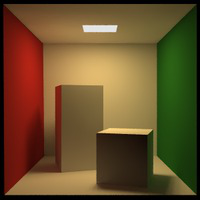
\includegraphics[width = .33\textwidth]{res/input3.png}};        &
    \node (o0) {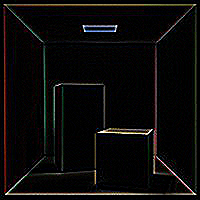
\includegraphics[width = .33\textwidth]{res/output3edge.png}};   \\
    \node (i1) {
\includegraphics[width = .33\textwidth]{res/input2.png}};        &
    \node (o1) {
\includegraphics[width = .33\textwidth]{res/output2blur3x.png}}; \\
    \node (i2) {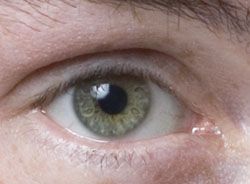
\includegraphics[width = .33\textwidth]{res/input6.png}};        &
    \node (o2) {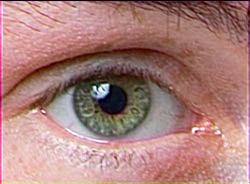
\includegraphics[width = .33\textwidth]{res/output6sharp.png}};  \\
  };

  \newcommand{\edgeMat}{$
    \begin{pmatrix}
       0 &  0 & -1 &  0 &  0 \\
       0 &  0 & -1 &  0 &  0 \\
      -1 & -1 &  8 & -1 & -1 \\
       0 &  0 & -1 &  0 &  0 \\
       0 &  0 & -1 &  0 &  0
    \end{pmatrix}
  $}

  \newcommand{\blurMat}{$
    \frac{1}{25}
    \begin{pmatrix}
       1 &  1 &  1 &  1 &  1 \\
       1 &  1 &  1 &  1 &  1 \\
       1 &  1 &  1 &  1 &  1 \\
       1 &  1 &  1 &  1 &  1 \\
       1 &  1 &  1 &  1 &  1
    \end{pmatrix}
  $}

  \newcommand{\sharpMat}{$
    \frac{1}{8}
    \begin{pmatrix}
      -1 & -1 & -1 & -1 & -1 \\
      -1 &  2 &  2 &  2 & -1 \\
      -1 &  2 &  8 &  2 & -1 \\
      -1 &  2 &  2 &  2 & -1 \\
      -1 & -1 & -1 & -1 & -1
    \end{pmatrix}
  $}

  \path ([yshift=1cm]i0.east) edge node[above] {edge detection} node[below] {\edgeMat}  ([yshift=1cm]o0.west);
  \path ([yshift=1cm]i1.east) edge node[above] {blurring}       node[below] {\blurMat}  ([yshift=1cm]o1.west);
  \path ([yshift=1cm]i2.east) edge node[above] {sharpening}     node[below] {\sharpMat} ([yshift=1cm]o2.west);
\end{tikzpicture}
\caption{Three examples of Kernels: edge detection, blurring and sharpening filters.}
\label{fig:kernels}
\end{figure}

The algorithm itself is relatively straightforward, as shown in
\RefCode{lst:kernelApply}. With the complete version available in
\RefApp{img_proc_code}, Leon is capable of showing that all array accesses and
arithmetic operations are valid, with two exceptions: the \InlineS{+=} and
\InlineS{*} on line 37 of \RefCode{lst:kernelApply}.

In order to prove that those two operations do not overflow, one should probably
add some constraints on the kernel size and its matrix content. For example, if
the size is assured to be at most 5 by 5 and all values of the matrix in the
range $[-10, 10]$, then only 16 bits are required to compute the new pixel
values before scaling it down as $5 * 5 * 10 * 256 < 2^{16}$. From this, we can
assume that in practice no overflow will occur when using 32-bit integers and
regular kernels.

\lstset{numbers=left}
\begin{Code}{Leon}{lst:kernelApply}{Implementation of the matrix convolution}
case class Kernel(size: Int, scale: Int, kernel: Array[Int]) {
  def apply(src: Image, dest: Image): Unit = {
    require(src.w == dest.w && src.h == dest.h)

    val size = src.w * src.h
    var i = 0
    (while (i < size) {
      dest.r(i) = apply(src.r, src.w, src.h, i)
      dest.g(i) = apply(src.g, src.w, src.h, i)
      dest.b(i) = apply(src.b, src.w, src.h, i)

      i += 1
    }) invariant (inRange(i, 0, size))
  }

  private def apply(channel: Array[Byte],
                    width: Int, height: Int, index: Int): Byte = {
    require(/*...*/)

    // Get the colour component at the given position
    def at(col: Int, row: Int):Int = {/*...*/} ensuring { inRange(_, 0, 255) }

    val mid = size / 2
    val i = index % width
    val j = index / width

    var res = 0
    var p   = -mid
    (while (p <= mid) {
      var q = -mid
      (while (q <= mid) {
        val kcol = p + mid
        val krow = q + mid
        val kidx = krow * size + kcol

        // Here, the += and * operation could overflow
        res += at(i + p, j + q) * kernel(kidx)

        q += 1
      }) invariant (inRange(q, -mid, mid + 1))
      p += 1
    }) invariant (inRange(p, -mid, mid + 1))

    clamp(res / scale, 0, 255).toByte
  }
}
\end{Code}
\lstset{numbers=none}

\subsection{Runtime Performances}

For this benchmark we compared exclusively the computational runtime of the
application, without taking into account the input and output processing times,
using several runtime environments. First, as a baseline, we ran the original
Scala source code on a JVM. Then, we used Leon and \GenC to convert it into C
code and generated four native versions using both Clang and GCC compilers, and
the \Inline{-O0} and \Inline{-O3} optimisation levels. In order to allow the JVM
to perform optimisation at runtime, each measurement was performed 50 times to
let the JIT compiler kick in. However, we did not attempt to optimise the
benchmark and exclude measures impacted by the garbage collector because we
strongly believe it is part of the language environment and therefore should be
accounted for.

To carry out this experiment, we set up a small API for benchmarks with an equivalent
implementation for C and Scala: it allows to measure in milliseconds the elapsed
time between two arbitrary points of a program. Given an source image, we
measured the time needed to allocate the memory for the output image and apply a
given kernel on the input image.

The benchmark was run on kernels and images of different sizes. To accommodate
for large images we used \emph{Variable Length Arrays}, despite being not
recommended by the MISRA guidelines, and increased the maximal stack size of our
Linux system using \Inline{ulimit}. The set of images ranges from very small,
200x200 pixels images to large ones with more than 22 megapixels. We used three
sizes of kernels: 1x1, 3x3 and 5x5 matrices. \RefTable{tab:improc_params}
reports these details.


\begin{table}[h]
\centering
\caption{Properties of input images and kernels.}
\label{tab:improc_params}
\begin{tabular}{@{}lll|l|ll@{}}
\toprule
Image         & Pixels    & Size   &  & Kernels  & Matrix \\ \midrule
input3.bmp    & 200x200   & 117 KB &  & identity & 1x1    \\
input6.bmp    & 250x184   & 136 KB &  & smooth   & 3x3    \\
input4.bmp    & 220x334   & 216 KB &  & emboss   & 3x3    \\
input2.bmp    & 512x288   & 433 KB &  & blur     & 5x5    \\
input1.bmp    & 384x480   & 541 KB &  & edges    & 5x5    \\
input5.bmp    & 512x384   & 577 KB &  & sharpen  & 5x5    \\
input7.bmp    & 1350x900  & 3.5 MB &  &          &        \\
input7big.bmp & 6000x4000 & 69 MB  &  &          &        \\ \bottomrule
\end{tabular}
\end{table}

\pagebreak
We used the following environment for this benchmark:
\begin{itemize}
\item Linux 4.8.0-42-generic x86\_64;
\item Intel(R) Core(TM) i7-6700 CPU @ 3.40GHz;
\item 4x 16GiB DIMM Synchronous 2133 MHz
\item Scala compiler/code runner version 2.11.6;
\item Java(TM) SE Runtime Environment (build 1.8.0\_121-b13) \&
      Java HotSpot(TM) 64-Bit Server VM (build 25.121-b13, mixed mode);
\item clang version 3.8.0-2ubuntu4 (tags/RELEASE\_380/final);
\item gcc version 5.4.0 20160609 (Ubuntu 5.4.0-6ubuntu1\~16.04.4);
\end{itemize}

We present in \RefFig{fig:improc-res} a subset of the results that highlights
the general trends of the measurements. In these results, we use the Scala
runtime as a baseline. In the first and second columns, we show the runtimes and
speedups for the second smallest and the largest image inputs, respectively,
using boxplots: the red lines identify the median runtime for each combination
of parameters. In the third column, we plotted the speedups across inputs, where
the smallest input is on the left of the x-axis and the largest on the right.
For each row of the figure, we present the result for a different kernel. The
first row shows the outcomes for the smallest filter, i.e. a 1x1 matrix, while
the second and third rows present the results for a 3x3 and 5x5 kernel matrix,
respectively. \emph{clang.0} corresponds to the runtime of the C code compiled
with Clang and no optimisation, while optimisation where turned on to the
compiler maximum level with \emph{clang.3}. The same applies for \emph{gcc.0}
and \emph{gcc.3}.

From this data, we note a few things. First, when no optimisation are enabled
for the native backends, both GCC and Clang perform equally bad compared to the
JVM runtime with a slowdown factor of roughly 2x. However, when optimisation are
turned on, GCC is capable of achieving speedups between 5x and 10x compared to
our JVM baseline. Clang is also able of significant runtime improvements as
well, but the generated assembly is slightly slower than the one generated by
GCC for this benchmark.

Then, the data shown in the third column of \RefFig{fig:improc-res} reveals that
the size on the input image does not affect the speedup factors, meaning that
all runtime environments scale similarly. The spike observed in the top right
graph is due to the runtime efficiency of the assembly code generated by GCC:
because the program runs extremely fast with the smallest image and kernel, the
unit used for runtime measurement might not be precise enough.

Additionally, when exploring the runtime data we saw that the JIT compiler did
not improve the performance of the JVM backend significantly throughout the
runs, the first and last runs taking approximately the same time. The variance
in the runtimes is therefore probably due to the garbage collector doing its
work.

In conclusion to this benchmark, it clearly appears that \GenC is capable of
producing efficient C code in comparison to the original Scala code. It follows
that using Leon to verify the safety of software does not implies slow runtimes.

We also modified the benchmark in order to be compatible with \emph{Scala
Native}\cite{scala_native} and therefore produce an alternative native runtime.
These modifications were surprisingly light and did not impact the main
algorithm. First, the I/O and timing facilities had to be rewritten using
functions from the standard C library, which resulted in a implementation close
to identical as the one produced by \GenC. Second, in order to use a stack
allocated memory, we replaced the \InlineS{Array[Byte]} by
\InlineS{native.Ptr[Byte]} and explicitly allocated the image data using
\InlineS{native.stackalloc[Byte](size)} function. However, and this can be
explained by the experimental nature of version 0.1 of \emph{Scala Native}, this
additional backend was slower than the C code generated by \GenC and compiled by
GCC or Clang. It is expected that the runtime performance of \emph{Scala Native}
will be significantly improved in upcoming updates and it would therefore be
relevant to run measurements for this benchmark again.


\begin{figure}[!h]
  \centerfloat
  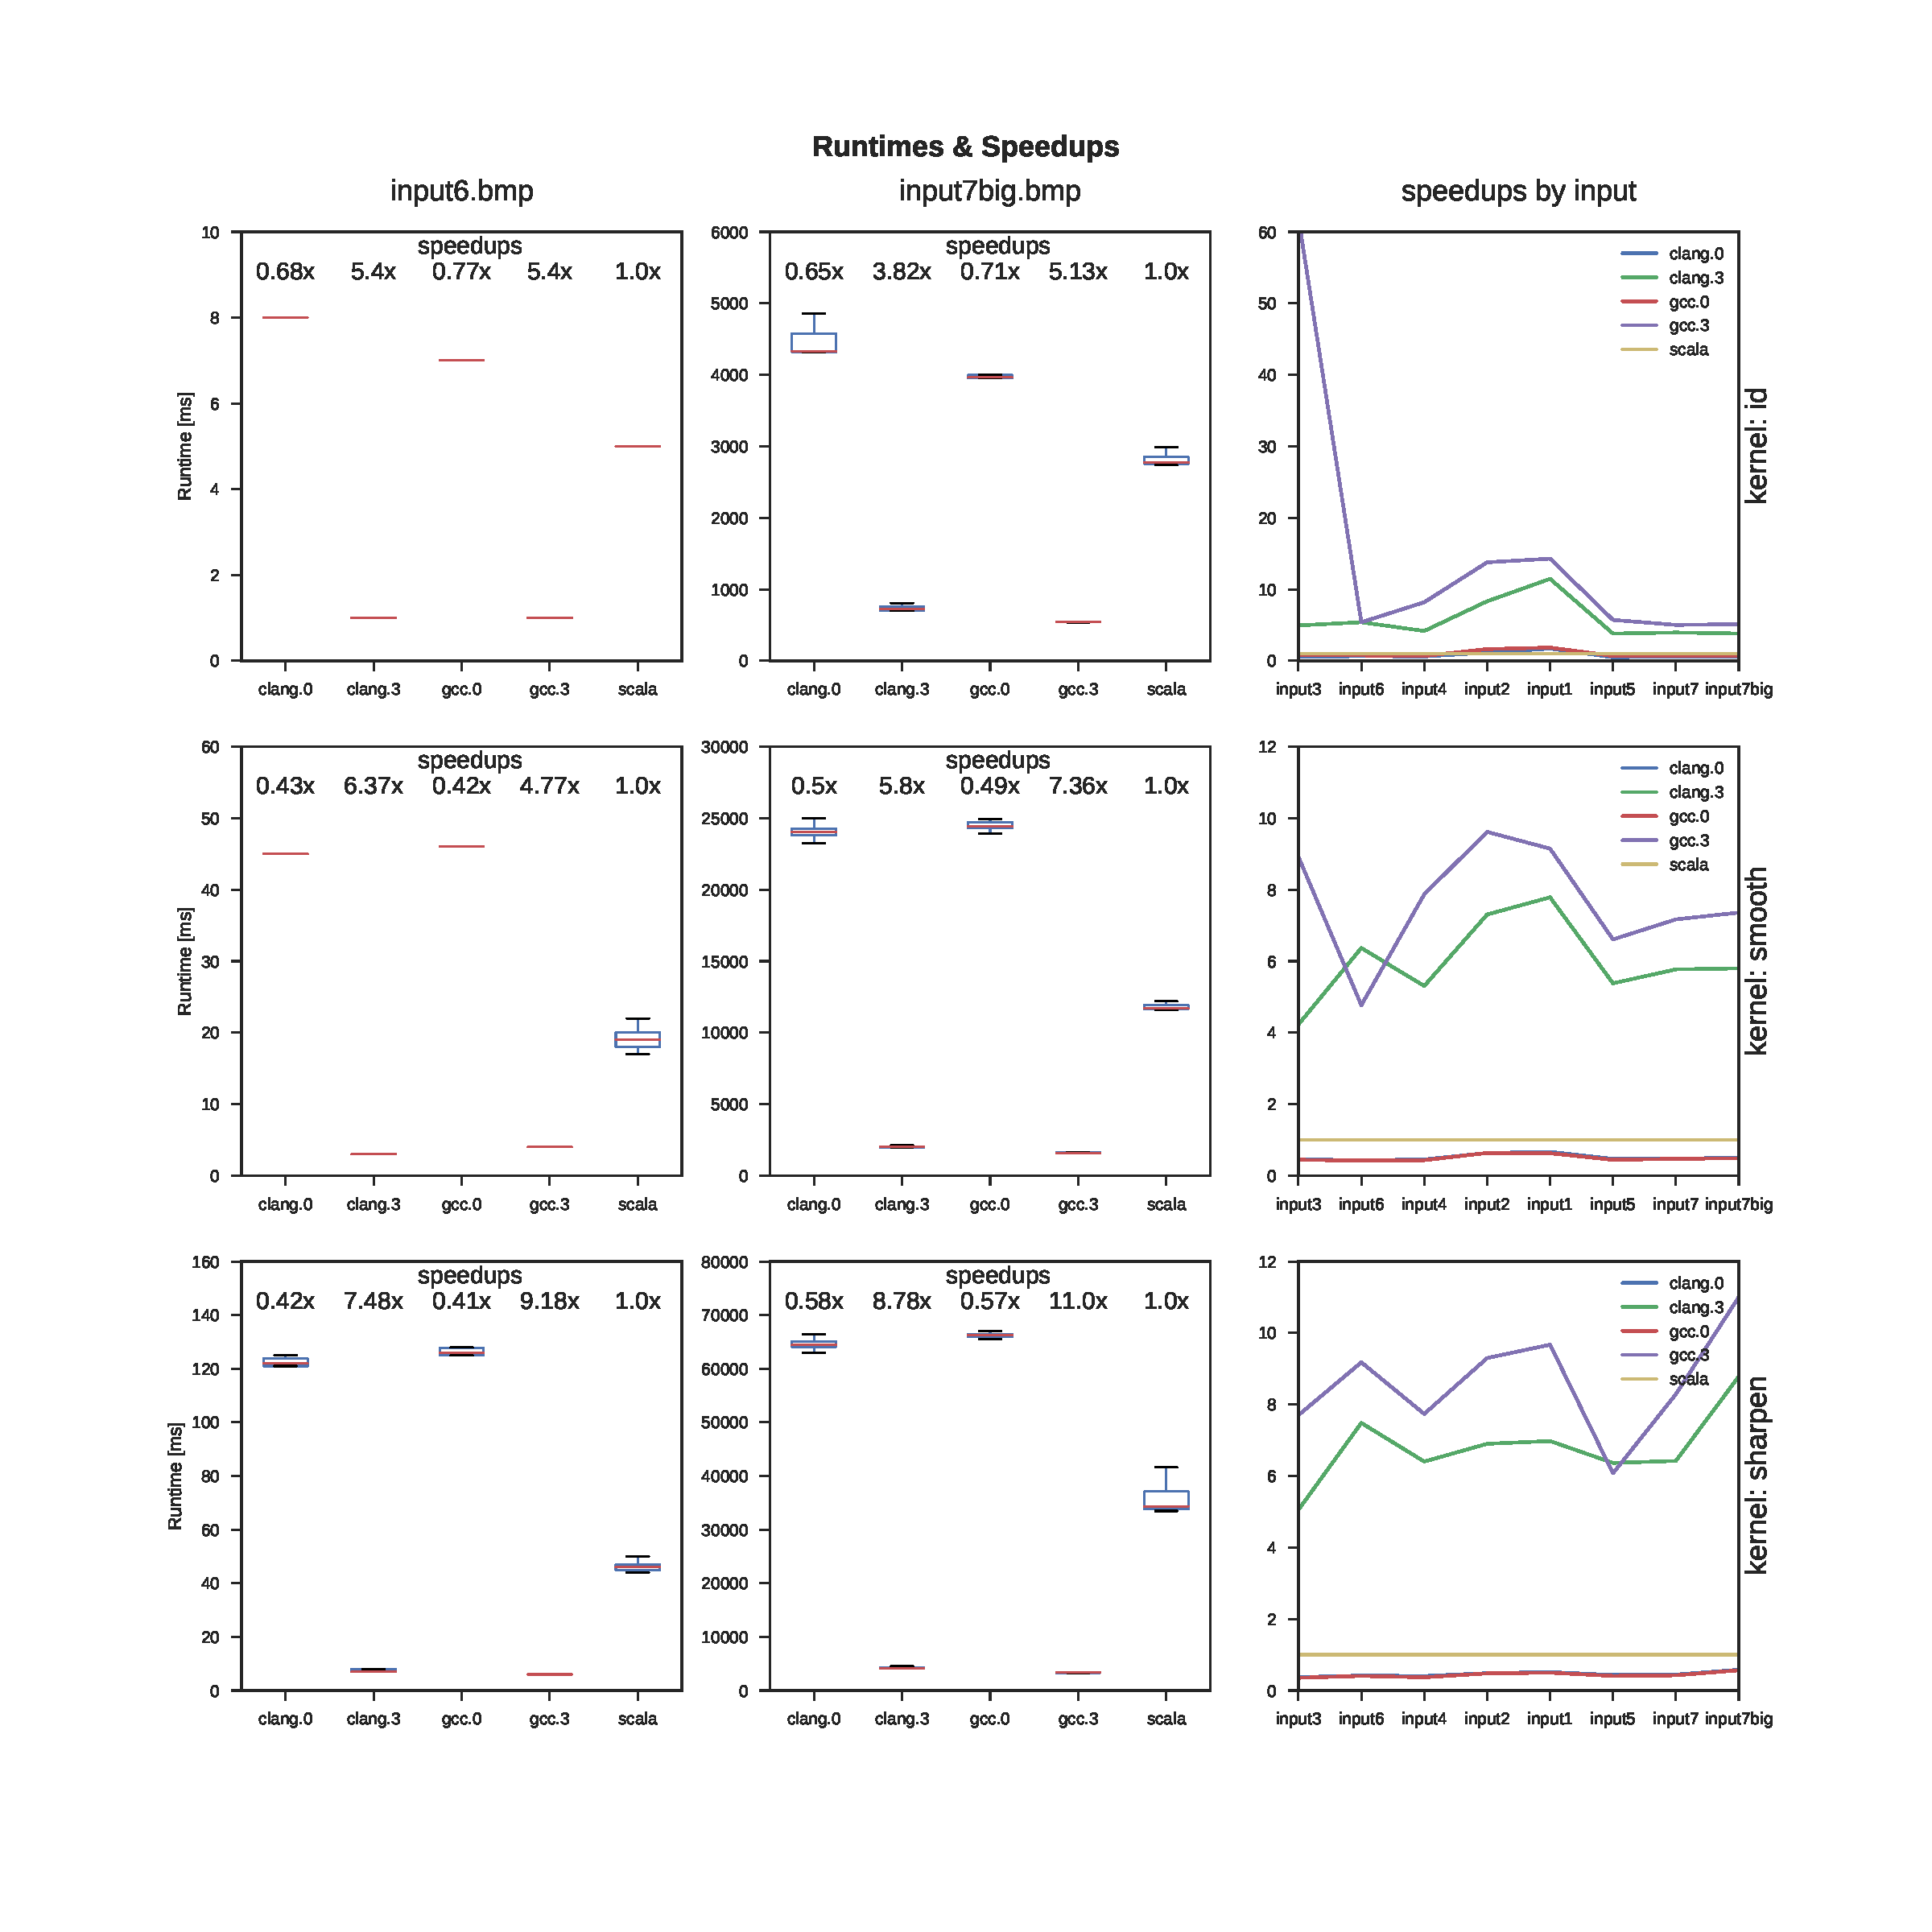
\includegraphics[width=1.25\textwidth]{res/improc_results.pdf}
  \caption{Results for the Image Processing Benchmark}
  \label{fig:improc-res}
\end{figure}


\section{Conclusion}
\label{conclusion}

The goals achieved in this project are multiple: we extended the verification
capabilities of Leon, significantly augmented the set of Scala programs that
\GenC can convert into C99 equivalent code while taking into account the MISRA
guidelines, and showed through two case studies that the generated programs are
significantly faster than the original Scala programs.

First, we introduced the ability to use \Inline{Byte} with Leon with the proper
integer promotion strategy used by Java and Scala. We also updated Leon to add
automatic verification for a wider range of potential integer overflows and to
detect unexpected behaviour in arithmetic expressions. Additionally, we
introduced an Input/Output API for standard streams and files, with a backend
for C99.

After carefully analysis the requirement imposed by the \emph{xlang} module
regarding aliasing we devised a stack-allocation based memory model, free of
dynamic allocation, that is capable of handling most form of mutability in class
hierarchies, and therefore imposes no requirement on heap memory management.

Not only did we introduce support for \Inline{Byte} and other primitive types,
but we managed to transpile generic types and functions into C code without
using language extensions nor introduce a runtime performance penalty. Next, we
presented a stronger model for normalisation of Scala code in order to properly
project the evaluation semantics of the input software onto the generate one. We
also significantly improved the safety of shift operations, thanks to a close
inspection of the Java 8 and C99 standards to understand exactly when an
expression is equivalent to another in both languages and, especially for C,
when undefined-behaviour can be triggered. With a better comprehension of the
limits of C programs we were able to use different integer types to workaround
some dangerous pitfalls by converting values from one to another type.

Furthermore, support for casts and membership tests within class hierarchies
were added as well as the ability to convert pattern matching expressions into
equivalent, imperative code. And in order to use stable and trusted C libraries
we designed an annotation systems to create proxy interface, providing a bridge
between Scala and C code.

One central aspect of this report is that we documented how \GenC is capable of
respecting, with very few exceptions, the strict MISRA Guidelines for critical
and embedded systems development, exposing when the verification tools of Leon
can be extremely beneficial and what the user is required to do to work his way
through full compliance.

We ended the discussion by using the LZW data compression and decompression
algorithm and an algorithm to apply filters on images to illustrate how
successfully \GenC can perform on real-life programs, although identifying some
limitations with nested arrays that are the consequences of our memory model.
Performance-wise, we showed that using Clang or GCC to compile the code
generated by Leon and \GenC, especially when using the compilers' clever
optimisations, result in runtime between 4x and 10x faster compared to the usual
JVM runtime offered by Scala, while being as safe as the source programs.


\section{Future Works}
\label{future_works}

We end the present document by opening the discussion on several points that
would benefit from further development:

\renewcommand{\labelitemi}{$\diamond$}
\begin{itemize}

\item Integrating optimisations in the generate code could be done by performing
some analysis on the AST to determine whether side-effect is present or not in a
given set of expressions; if expressions are all pure the normalisation
introduced in \RefSec{normalisation} could be avoided, generating simpler
programs that C compilers could optimise more easily. Additionally, some
\InlineC{if} statements could be transformed into \InlineC{switch} statements
when, for example, the branching only depends on an \InlineC{enum} value.

Performance benefit from such optimisations are however hard to estimate because
nowadays C compilers do already perform some aggressive optimisations when asked
to.

\item Resource inference introduced by Orb \cite{Madhavan2014} to deal more
efficiently with imperative programs, giving developers a good analysis of the
memory requirement for their generated C99 programs, but also in term of speed
were an accurate execution model be elaborated for a given hardware system.

\item Adding an extra layer to the I/O library component of Leon to
automatically close file handle when they go out of scope. This could be
implemented with an inlined and curried function, similar to the one exposed
below, fundamentally using the same trick than for \InlineS{Option} discussed in
\RefSec{library}.

\begin{ShortCode}{Leon}
@inline
def withFile(filename: String)
            (onSuccess: FileInputStream => Unit): Boolean = {
  val fis = FileInputStream.open(filename)
  if (fis.isOpen) {
    onSuccess(fis)
    fis.close()
    true
  } else false
}
\end{ShortCode}

Alternatively, two callback functions could be passed to \InlineS{withFile} and
a generic return type could be inferred from them. But in any case the passed
functions could only be anonymous lambdas as higher order functions remains a
complex concept when expressed in C, especially while maintaining the semantics
of Scala.

\item With upcoming updates to the xlang module \cite{xlang}, the aliasing
restrictions are expected to be slightly relaxed, essentially allowing a
variable, or one of its member, to be aliased by another if only one of them is
used subsequently.

\begin{ShortCode}{Leon}
def foo(x: MutableType) = {
  val y = x // Currently illegal but planned to be valid
  bar(y)    // as x is not used after y is created.
}
\end{ShortCode}

Such modification of the anti-aliasing rules would require a reassessment of how
\GenC handle mutability to determine whether the translation process remains
sound.

\item The memory model presented in \RefSec{memory_model} is known to suffer
from one flaw illustrated in \RefCode{lst:validXlang}. Two opposite updates are
interesting at this point. The first would be to notify the user when \GenC
detects code that it cannot properly handle, possibly stopping the translation
process.

The other alternative would be to considerably change the ownership model used
by \GenC to represent types in two fashions: \emph{owner} and \emph{reference}.
The former would have exclusively value attributes and own them. The latter
would be bound to an \emph{owner} and have references for its mutable fields.
Additionally, we should be able to convert an \emph{owner} to a \emph{reference}
but not vice-versa. This framework allows passing mutable tuples or case classes
to functions and respect aliasing (and therefore propagates mutation) when
functions can return only the \emph{owner} variant of a type.

Applied to \RefCode{lst:validXlang}, instead of producing \RefCode{lst:badcopy}
\GenC could generate a program along these lines:

\begin{ShortCode}{C99}
typedef struct { int x; } A;
typedef struct { A   a; } B_owner;
typedef struct { A*  a; } B_ref;

static void update(A* a) {
  updateB((B_ref) { .a = a });
  /* no copy:            ^  */
}
\end{ShortCode}

Such modification of the type translation and representation however would
require a full analysis, assessing notably if the augmentation of types and type
conversions impacts the generated C99 code in an undesirable way. Moreover, the
impact of the relaxed aliasing rules described above should be taken into
account when solving this limitation.

\item In order to make the process to have MISRA compliant C code developers
using \GenC need to pay attention to several points discussed in
\RefSec{user_responsibility}. Documenting and keeping track of how each point is
taken care of is obviously a tedious task when done solely manually. However,
for several points Leon and \GenC could emit warnings and instruct users how to
solve specific issues. We list here several points of interest for a linter-like
report:

  \begin{enumerate}

  \item Directive 4.7 and Rule 17.7 both ask that value returned by function
  should be used~-- the former specifically address error values signalled by
  functions. Automatically reporting when a value is not read should be possible
  locally to each function body.

  \item Identifying systematically unreachable or dead code would directly help
  fulfilling Rules 2.1 and 2.2.

  \item Side effect present when initialising arrays, objects or in operands
  would make it trivial to check for compliance to Rules 13.1 and 13.5.

  \item Similarly, the benefits of reporting places in the user code where an
  identifier shadows another one are twofold: it would make Rules 5.2, 5.3 and
  5.7 obsolete and this would allow \GenC to avoid using complex postfixes on
  identifiers in many places, consequently making the generated C code looking
  more similar to the original Scala code.

  \item Using simple checks on the AST Leon and \GenC could determine whether
  all \InlineS{if} statements have an \InlineS{else} branch in order to satisfy
  Rule 15.7. Similarly, when multiple \InlineC{return} expressions are inserted
  by \GenC a warning could be emitted for Rule 15.5.

  \item Finally, having the ability to detect overflows in \emph{constant
  expression} within Leon would allow use to warn the user when Rule 12.4 is not
  respected.

  \end{enumerate}

\end{itemize}


\appendix

\section{Operator Equivalence Table}
\label{ops_checklist}

\newcommand{\VHeader}[1]{\rotatebox{90}{\textbf{#1}}}
%% ASSUMING THIS IS THE LAST LIST IT SHOULD BE FINE TO DO THIS
\renewcommand{\labelitemi}{$\diamond$}
\setlength{\leftmargini}{1em}

Here we briefly present an analysis of the different arithmetic operators
present in Java and C, highlighting the differences of semantics and behaviour
as well as identifying the legal range of values.

The first column determines whether the C99 operator presented in the second one
takes one argument (\emph{unary}) or two arguments (\emph{binary}). The
arguments are denoted by \emph{rhs} and \emph{lhs}, which stand for right- and
left-hand side. The seventh column contains the closest Java operator. The valid
range of values is detailed in columns four and five for the C99 standard and in
columns nine and ten for the Java environment. We refer in columns three and
eight to which sections of the C Standard \cite{c99} and Java Standard
\cite{java8}, respectively, define the exact semantic of the operators.

Then we highlight in the last column the main differences between the C and Java
operators. And finally, in the sixth column we use four symbols that specify
under which condition the C99 and Java semantics of the operator are equivalent.
Their respective meaning is as follows when the operations are carried out on
32-bit integers:

\newcommand{\SemEqual}{\checkmark}
\newcommand{\SemOverflow}{$\mathcal{O}$}%$\vee$
\newcommand{\SemStrict}{$\mathcal{S}$}%\textdagger
\newcommand{\SemNA}{\ding{53}}

\begin{description}[style=nextline]
\item[\SemEqual] The two semantics are completely equivalent.
\item[\SemOverflow] The semantics are equivalent when no overflow occur.
\item[\SemStrict] Under \Inline{--strict-arithmetic} verification mode the two
are identical.
\item[\SemNA] There is no direct equivalence between the operator.
\end{description}

\clearpage
% \newpage\null\thispagestyle{empty}\newpage
\begin{landscape}

\begin{tabular}{@{}lllp{3em}l|l|llll|p{7cm}@{}}
\toprule
\VHeader{Category} & \VHeader{C operator} & \VHeader{C99} & \VHeader{lhs range} & \VHeader{rhs range} & \VHeader{Semantic} & \VHeader{Java operator} & \VHeader{Java 8} & \VHeader{lhs range} & \VHeader{rhs range} & \VHeader{Comment} \\ \midrule

unary & \Inline{+} & 6.5.3.3 & any int & N/A & \SemEqual & \Inline{+} & 15.15.3 & any int & N/A & Not in Leon \\

unary & \Inline{-} & 6.5.3.3 & all but \Inline{INT_MIN} & N/A & \SemOverflow & \Inline{-} & 15.15.4 & any int & N/A & In Java \Inline{-INT_MIN == INT_MIN} \\

binary & \Inline{*} & 6.5.5 & any int & any int & \SemOverflow & \Inline{*} & 15.17.1 & any int & any int & \\

binary & \Inline{/} & 6.5.5 & any int & non-zero & \SemOverflow & \Inline{/} & 15.17.2 & any int & non-zero &
\vspace{-1.5ex}
\begin{itemize}[nosep]
\item C99 defines division in the same fashion as Java and C++11.
\item In Java \Inline{INT_MIN / -1 == INT_MIN}.
\item \Inline{INT_MIN / -1} overflows in C.
\end{itemize} \\

binary & \Inline{\%} & 6.5.5 & any int & non-zero & \SemStrict & \Inline{\%} & 15.17.3 & any int & non-zero &
\vspace{-1.5ex}
\begin{itemize}[nosep]
\item \Inline{MIN_INT \% -1} is undefined in C11.
\item It is unclear in C99~\cite{regehr}.
\item In Java the result is defined to be 0.
\end{itemize} \\

binary & \Inline{+} & 6.5.6 & any int & any int & \SemOverflow & \Inline{+} & 15.18.2 & any int & any int & \\

binary & \Inline{-} & 6.5.6 & any int & any int & \SemOverflow & \Inline{-} & 15.18.2 & any int & any int & \\ \midrule

unary & \Inline{\~} & 6.5.3.3 & any int & N/A & \SemEqual & \Inline{\~} & 15.15.5 & any int & N/A & \\

binary & \Inline{\&} & 6.5.10 & any int & any int & \SemEqual & \Inline{\&} & 15.22.1 & any int & any int & \\

binary & \Inline{^} & 6.5.11 & any int & any int & \SemEqual & \Inline{^} & 15.22.1 & any int & any int & \\

binary & \Inline{|} & 6.5.12 & any int & any int & \SemEqual & \Inline{|} & 15.22.1 & any int & any int & \\ \bottomrule

\end{tabular}


\begin{tabular}{@{}lp{3em}lp{4em}l|l|p{2em}lll|p{7cm}@{}}
\toprule
\VHeader{Category} & \VHeader{C operator} & \VHeader{C99} & \VHeader{lhs range} & \VHeader{rhs range} & \VHeader{Semantic} & \VHeader{Java operator} & \VHeader{Java 8} & \VHeader{lhs range} & \VHeader{rhs range} & \VHeader{Comment} \\ \midrule

binary & signed \Inline{<<} & 6.5.7 & see comment & $[0,31]$ & \SemStrict & \Inline{<<} & 15.19 & any int & any int &
\vspace{-1.5ex}
\begin{itemize}[nosep]
\item In Java, only the 5 lowest-order bits of rhs are used (range $[0,31]$).
Moreover, the bits are always shifted as one would expect.
\item In C, assuming rhs is in $[0,31]$, we also need to have $lhs * 2^{rhs}$ in
$[0, 2^{31}-1]$; otherwise the behaviour is undefined.
\end{itemize} \\

binary & unsigned \Inline{<<} & 6.5.7 & any unsigned int & $[0,31]$ & \SemStrict & \Inline{<<} & 15.19 & any int & any int &
\vspace{-1.5ex}
\begin{itemize}[nosep]
\item Assuming rhs is in $[0,31]$, the unsigned version of << in C99 is equivalent to Java's.
\item However, converting back from unsigned integer is implementation defined!
\end{itemize} \\

binary & signed \Inline{>>} & 6.5.7 & any non-negative int & $[0,31]$ & \SemNA & \Inline{>>} or \Inline{>>>}\footnotemark & 15.19 & any int & any int &
\vspace{-1.5ex}
\begin{itemize}[nosep]
\item In Java, only the 5 lowest-order bits of rhs are used (range $[0,31]$).
\item Moreover, in Java, \Inline{>>} will sign-extend lhs while \Inline{>>>} will zero-extend lhs.
\item In C99, signed integer right shift is implementation defined for negative integers.
\end{itemize} \\

binary & unsigned \Inline{>>} & 6.5.7 & any unsigned int & $[0,31]$ & \SemStrict & \Inline{>>>} & 15.19 & any int & any int &
\vspace{-1.5ex}
\begin{itemize}[nosep]
\item In Java, only the 5 lowest-order bits of rhs are used (range $[0,31]$) and lhs will be zero-extended.
\item In C99, assuming rhs is in $[0,31]$, basically, lhs gets zero-extended.
\end{itemize} \\ \bottomrule

\end{tabular}
\footnotetext{Depending on the sign of lhs.}


\section{LZW Implementations}
\label{LZW_code}

For completeness, we give print here our two implementations of LZW written in
Scala as well as the C99 programs generated by \GenC. The sources are also
available at \url{https://github.com/mantognini/GenC}.

\subsection{Scala Source}

\subsubsection*{Design A}
\label{lzw_impl_scala_a}
\lstinputlisting[language=Leon, style=LongCode]{case_studies/LZW/LZWa.scala}

\clearpage
\subsubsection*{Design B}
\label{lzw_impl_scala_b}
\lstinputlisting[language=Leon, style=LongCode]{case_studies/LZW/LZWb.scala}

\clearpage
\subsection{Generated C99 Code}

\subsubsection*{Design A}
\label{lzw_impl_c_b}

The generated code is unfortunately too long to decently fit in this annex for
reasons detailed in \RefSec{lzw_dictionaries}. It can however be accessed here:
\url{https://github.com/mantognini/GenC}.

\subsubsection*{Design B}
\label{lzw_impl_c_b}
\lstinputlisting[language=C99, style=LongCode]{case_studies/LZW/LZWb.c}

\section{Image Processing Implementation}
\label{img_proc_code}

For completeness, we give print here our implementation of the Image Processing
case study written in Scala as well as the C99 program generated by \GenC. The
sources are also available at \url{https://github.com/mantognini/GenC}.

\subsection{Scala Source}
\label{img_proc_scala}
\lstinputlisting[language=Leon, style=LongCode]{"case_studies/Image Processing/ImageProcessing.scala"}

\clearpage
\subsection{Generated C99 Code}
\label{img_proc_c}
\lstinputlisting[language=C99, style=LongCode]{"case_studies/Image Processing/ImageProcessing.c"}

\end{landscape}

\clearpage

\bibliographystyle{ieeetr}
\bibliography{report}

\end{document}

% vim: spell spelllang=en_gb
% vim: set tabstop=2 softtabstop=2 shiftwidth=2 textwidth=80: %
% vim: set ai nocin nosi indk=: %
% vim: set inde=: %

